
\section{A motivation for Bayesian methods}

Background from \url{https://cims.nyu.edu/~andrewgw/caseforbdl.pdf}

This is mostly to share ideas of applications for (mostly) Bayesian Deep Learning, apart from the usual stuff in adversarial ML. The idea of these applications is to motivate the research in BDL and to be used as experiments in future Bayesian papers and the thesis.

\begin{itemize}
    \item Active Learning: in order to choose new points for labeling, we need to compute entropies of predictions + acquisition function (AF) as in \url{https://arxiv.org/abs/1906.08158}. With better uncertainty estimates the performance should be higher for a given AF. This should be easy to implement, since experiments are MNIST based.
    \item The retina benchmark from \url{http://www.cs.ox.ac.uk/people/angelos.filos/publications/diabetic_retinopathy_diagnosis.pdf}.
    \item VOED: in \url{https://arxiv.org/pdf/1903.05480.pdf} authors propose an amortized variational approximation.
    \item VIREL: a framework similar to MERL from \url{https://arxiv.org/pdf/1811.01132.pdf}.
    \item Deep Image Prior: apart from the prior, the Bayesian version avoids overfitting for image reconstruction tasks. \url{https://zpascal.net/cvpr2019/Cheng_A_Bayesian_Perspective_on_the_Deep_Image_Prior_CVPR_2019_paper.pdf}
\end{itemize}

\subsection{Arguments}

\begin{itemize}
    \item In defence of Bayesian DL, focusing on marginalization (in the predictive distribution): \url{https://cims.nyu.edu/~andrewgw/caseforbdl.pdf}. Related to that (specially in the critique of BNN priors, see \url{https://www.reddit.com/r/MachineLearning/comments/eqdad9/d_a_sober_look_at_bayesian_neural_networks/}
    
    \item \url{https://oatml.cs.ox.ac.uk/blog/2020/04/22/Beyond-Discrete-Support-in-Large-Scale-Bayesian-Deep-Learning.html} criticises discrete support methods, such as MCMC, in continual settings. But this is a setting similar to SMC, so a resampling step solves the problem...
\end{itemize}

\section{A case study in the retail sector using Bayesian time series models}\label{sec:dlms}

\subsection{Context}

It is widely acknowledged that a firm's expenditure  on advertising has a positive effect on sales \parencite{assmus1984advertising, tellis2007advertising, luo2012does, wiesel2011practice}. However, the exact relationship between them remains a moot point, see \parencite{tellis2009generalizations} for a broad survey. Since Dorfman and Steiner's \parencite{dorfman1954optimal} seminal work\, several models have been proposed to pinpoint this relationship, although consensus on the best approach has not been reached yet. Two diverging model-building schools seem to dominate the marketing literature \parencite{little1979aggregate}: \emph{a priori} models rely heavily on intuition and are derived from general principles, although usually with a practical implementation on mind (\parencite{nerlove1962optimal}, or \parencite{vidale1957operations} and \parencite{little1975brandaid} \emph{inter alia}); and  \emph{statistical} or \emph{econometric} models, which usually start from a specific dataset to be modelled (e.g. \parencite{assmus1984advertising}). Here we will mostly rely on the first type of models, \emph{viz.} that of Nerlove-Arrow \parencite{nerlove1962optimal}, which extends  Dorfman and Steiner to a dynamic setting \parencite{bagwell2007economic} and adapts seamlessly to the \emph{state-space} or \emph{structural} time series approach.



Bayesian structural time series models \parencite{scott2014predicting}, in turn, have positioned themselves in the past few years as very effective tools  not only for analysing marketing time-series, but also to throw light into more uncertain terrains like  causal impacts, incorporating \emph{a priori} information into the model, accommodating multiple sources of variations or supporting variable selection. Although the origins of this formalism can be traced back to the 1950's in engineering problems of filtering, smoothing and forecasting, first with Wiener \parencite{wiener1949extrapolation} and specially with Kalman \parencite{kalman1960new}, these problems can also be understood from the perspective of estimation in which a vector valued time series $\{ X_0, X_1, X_2, \ldots\}$ that we wish to estimate (the \emph{latent} or \emph{hidden} states) is observed through a series of noisy measurements $\{ Y_0, Y_1, Y_2, \ldots\}$. This  means that, in the Bayesian sense, we want to compute the joint posterior distribution of all the states given all the measurements \parencite{sarkka2013bayesian}. The ever-growing computing power and release of several programming libraries  in the last few years like \parencite{petris2010r, scott2016bsts} have in part alleviated the difficulties in the implementation  that this formalism suffers, making these methods broadly known and used. This family of models have been used successfully to, e.g., model financial time series data \parencite{doi:10.1002/asmb.428}, infer causal impact of marketing campaigns \parencite{brodersen2015inferring}, select variables and nowcast consumer sentiment  \parencite{scott2015bayesian}, or for predicting other economic time series models like unemployment \parencite{scott2014predicting}.

We use the formalism of Bayesian structural time-series models to formulate a robust model that links advertising expenditures with weekly sales. Due to the flexibility and modularity of the model, it will be well suited to generalization to various markets or situations. Its Bayesian nature also adapts smoothly to the issue of introducing prior information. The formulation of the model allows for non-gaussian innovations of the process, which will take care of the heavy-tailedness of the distribution of sales increases. We also discuss how the forecasts produced by this model can help the manager into allocating the advertising budget. The decision space is reduced to a one dimensional curve of Pareto optimal strategies for  two moments of the forecast distribution (expected return and variance).

%The paper is organized as follows: after a brief review of the most usual marketing models and the formalism of structural time series in section 2, we define the model to be used to fit the data. The experimental setup will be detailed in section 3. Section 4 provides a discussion in which alternative models will be compared and also possible uses of this model in the industry. A brief summary and ideas for further research are detailed in section 5.



\subsection{Theoretical background and model definition}


\paragraph{The Nerlove-Arrow model.}


Numerous formulations of aggregate advertising response models exist in the  literature, e.g. \parencite{little1979aggregate}. The model of Nerlove and Arrow \parencite{nerlove1962optimal} extends the Dorfman-Steiner model to cover the situation in which current advertising expenditures affect future product demand; it is parsimonious and is considered as a standard in the quantitative marketing community. We use it as our starting point.

In this model, advertising expenditures are considered similar in many ways to investments in durable plant and equipment, in the sense that they affect the present and future character of output and, hence, the present and future net revenue of the investing firm. The idea is to define an ``advertising stock'' called \emph{goodwill}  $A(t)$ which seemingly summarizes the effects of current and past advertising expenditures over demand. Then, the following dynamics is defined for the goodwill

\begin{equation}\label{eq:NA}
\frac{dA}{dt} = qu(t) - \delta A(t),
\end{equation}
where $u(t)$ is the advertising spending rate (e.g., euros or gross rating points per week), $q$ is a parameter that reflects the advertising quality (an effectiveness coefficient) and $\delta$ is a decay or forgetting rate. \emph{Goodwill} then increases linearly with  advertisement expenditure but decreases also linearly due to forgetting. %Note that the last term breaks the linearity of the model, i.e. it prevents from achieving arbitrary large goodwill by increasing the advertising expenditure.

Several extensions and modifications have been proposed to this simple model: it can include a limit for potential costumers \parencite{vidale1957operations}, a non-linear response function to advertise expenditures \parencite{little1975brandaid}, wear-in and wear-out effects of advertising \parencite{naik1998planning},  interactions between different advertising channels \parencite{bass2007wearout}, among others. Still, for most  tasks, the  Nerlove-Arrow model remains as a simple and solid starting point. 

\paragraph{Bayesian structural time series models.}


\emph{Structural time series models} or \emph{state-space models} provide a general formulation that  allows a unified treatment of virtually any linear time series model through the Kalman filter and the associated smoother. Several handbooks \parencite{durbin2012time, petris2009dynamic, sarkka2013bayesian, west1998bayesian} discuss this topic in depth. We will  present a few salient features that concern our modelling problem. For further details, the reader may check the aforementioned handbooks. 

The state-space formulation of a time series consists of two different equations: the \emph{state} or \emph{evolution equation} which determines the dynamics of the state of the system as a first-order Markov process ---\,usually parametrized through \emph{state} variables\,--- and an \emph{observation} or \emph{measurement  equation} which links the latent state with the observed state. Both equations are also affected by noise.
\begin{equation}\label{eq:st}
\theta_{t} = G_t \theta_{t-1} + \epsilon_t \qquad \epsilon_t \sim \mathcal{N}(0, W_t).
\end{equation}
The states ($\theta_t$) are not generally observable, but are linked to the \emph{observation variables} $Y_t$ through the \emph{observation equation}:
\begin{equation}\label{eq:obs}
Y_t = F_t \theta_t + \epsilon'_t \qquad \epsilon'_t \sim \mathcal{N}(0, V_t).
\end{equation}
We denote by $\mathbf{\theta}_t$ the $m\times1$ \emph{state vector} describing the inner state of the system, by $G_t$ the $m\times m$ matrix that generates the dynamics, and by $ \epsilon_t $ a $g\times 1$ vector of serially uncorrelated disturbances with mean zero and covariance matrix $W_t$. $F_t$ is the $1\times m$ matrix that links the inner state to the observable, and $V_t \in \mathbb{R}^+$ is the variance of $\epsilon'_t $, the random disturbances of the observations.



%The dependence structure is depicted in Figure \ref{fig:ss}. Since the state sequence $\{ \theta_t\}$ is a Markov chain,  each observation $Y_t$ is independent on past observations conditioned on  state $\theta_t$. 

%\begin{figure}[h]
%\centering
%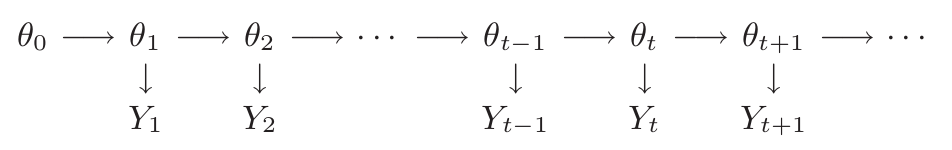
\includegraphics[scale=0.35]{figures/ss_model}
%\caption{Dependence structure for a DLM.}\label{fig:ss}
%\end{figure}


The specification of the state-space system is completed by assuming that the initial state vector $\theta_0$ has mean $\mu_0$ and a covariance matrix $\Sigma_0$ and it is uncorrelated with the noise. The problem then consists of \emph{estimating the sequence of states $\{\theta_1, \theta_2, \ldots\}$ for a given series of observations $\{y_1, y_2, \ldots\}$} and whichever other structural parameters of the transition and observation matrices. State estimation is readily performed via the \emph{Kalman filter};  different alternatives however arise  when structural parameters are unknown. In the classical setting, these are estimated using maximum likelihood. In the Bayesian approach, the probability distribution about the unknown parameters is updated via Bayes Theorem. If exact computation through conjugate priors is not possible, the probability distributions before each measurement are updated by approximate procedures such as Markov chain Monte Carlo (MCMC) \parencite{scott2014predicting}. 

The Bayesian approach offers several advantages compared to classical methods. For instance, it is natural to incorporate external information through the prior distributions. In particular, this will be materialized in Section \ref{sec:s_s} where expert information can be incorporated through the spike and slab prior. Another useful advantage is that, due to the Bayesian nature of the model, it is straightforward to obtain predictive intervals through the predictive distribution (see Section \ref{s:MCMC}).


\paragraph{Model specification.}\label{sec:model}



%\paragraph{State-space formulation.}


The continuous-time Nerlove-Arrow model must be first cast in discrete time so as to formulate our model in state-space. From equation (\ref{eq:NA}), we get:

$$
A_t =  (1-\delta) A_{t-1} + q u_{t-1} + \epsilon_t 
$$
where $A_t$ is the \emph{goodwill} stock, $u_t$ is the advertising spending rate, $q$ is the effectiveness coefficient and the random disturbance $\epsilon_t$  captures the net effects of the variables that affect the goodwill  but cannot be modelled explicitly.  This discrete counterpart of Nerlove-Arrow is a distributed-lag structure with geometrically declining weights, i.e., a \emph{Koyck model} \parencite{clarke1976econometric, koyck1954distributed}. Since in our setting the model includes the effect of $k$ different channels in the goodwill, we modify the previous equations to:

$$
A_t =  (1-\delta) A_{t-1} + \sum_{i=1}^k q_i u_{i(t-1)} + \epsilon_t 
$$

Now, following  (\ref{eq:st}) and (\ref{eq:obs}), the discrete-time Nerlove-Arrow model in state-space form will read:
\begin{description}

\item[Evolution equation:]

\begin{equation} \label{eq:NA_st}
\theta_{t} = G_t \theta_{t-1} +  \epsilon_t \qquad \epsilon_t \sim \mathcal{N}(0, W_t),   
\end{equation}
\noindent where
\begin{equation*} 
\theta_{t}  = \begin{bmatrix} A_t  \\ q_1 \\  \vdots \\q_k \end{bmatrix}
, \quad
G_t =  \begin{bmatrix}
   (1- \delta) & u_{1(t-1)} &  \ldots & u_{k(t-1)} \\
   0 & 1 &   \ldots & 0 \\
   \vdots  &   \vdots & \ddots & \vdots \\
   0 & 0 &  \ldots & 1 \\
   \end{bmatrix}.
%, \quad
% H_t =    \begin{bmatrix} 1  \\ 0 \\ \vdots \\ 0 \end{bmatrix}
\end{equation*}


Note that the $q_i$ are constant over time and that the matrix $G_t$ depends on the known inversion levels at time $t-1$ and on an unknown parameter ($\delta$) to be estimated from the data.

 \item[Observation equation:]
 
 \begin{equation} \label{eq:NA_obs}
 Y_t = F_t \theta_t + \epsilon'_t \qquad \epsilon'_t \sim \mathcal{N}(0, V_t)  
 \end{equation}

 
 where $Y_t$ are the observed sales at time $t$ and $F_t = \begin{bmatrix} 1,  & 0 , & \ldots, & 0 \end{bmatrix}$.
% + \sum_{i=1}^p \beta_iX_{i,t}
\end{description}


\paragraph{Modularity and additional structure.}

The above model is very flexible in the sense that it can be defined \emph{modularly},  in as much as different hidden states evolve independently of the others (\emph{i.e.} the evolution matrix can be cast in block-diagonal form). This greatly simplifies their implementation and allows for simple building-blocks with characteristic behavior. Typical blocks specify trend and seasonal components ---\,which can be helpful to discover additional patterns in the time series--- or explanatory variables that can be added to further reduce  uncertainty in the model and bridge the gap between time series and regression models. Via the \emph{superposition principle} \parencite[Chapter 3]{petris2009dynamic} we could include additional blocks in our model:

$$
Y_t = Y_{NA, t} + Y_{R, t} + Y_{T, t} + Y_{S, t}
$$
where $Y_{NA, t}$ corresponds to the discretized Nerlove-Arrow equation, defined in (\ref{eq:NA_st}) and (\ref{eq:NA_obs}); $Y_{R, t}$ is a regression component; containing the effects of  external explanatory variables $X_t$; $Y_{T, t}$ is a trend component or a simpler local level component; and $Y_{S, t}$ is a seasonal component.

\paragraph{Regression components. Spike and slab variable selection.}\label{sec:s_s}

To take into account the effects of external explanatory variables such as the weather or sport events, a  regression component can be easily incorporated into the model through

$$
Y_{R,t} = X_t \beta + \epsilon_t,
$$
where the state $\beta$ is constant over time to favor parsimony.

A spike and slab prior \parencite{mitchell1988bayesian} is used for the  regression component, since it can incorporate \emph{prior information} and also facilitate variable selection. This is specially useful for models with a large number of regressors, a typical setting in business scenarios.
Let $\gamma$ denote a binary vector that indicates whether the regressors are included in the regression. Specifically, $\gamma_i = 1$ if and only if $\beta_i \neq 0$. The subset of $\beta$ for which $\gamma_i = 1$ will be denoted $\beta_{\gamma}$. Let $\sigma^2_{\epsilon}$ be the residual variance from the regression part. The spike and slab prior \parencite{george1997approaches} can be expressed as
$$
p(\beta, \gamma, \sigma^2_{\epsilon}) = p(\beta_{\gamma} | \gamma, \sigma^2_{\epsilon})p(\sigma^2_{\epsilon} | \gamma)p(\gamma).
$$
A usual choice for the $\gamma$ prior is a product of Bernoulli distributions:

$$
\gamma \sim \Pi_i \pi_i^{\gamma_i}(1-\pi_i)^{1-\gamma_i}.
$$
The manager of the firm may elicit these $\pi_i$ in various ways. A reasonable choice when detailed prior information is unavailable is to set all $\pi_i = \pi$. Then, we may specify an expected number of non-zero coefficients by setting $\pi = k/p$, where $p$ is the total number of regressors. Another possibility is to set $\pi_i = 1$ if the manager believes that the $i-$th regressor is crucial for the model. %For instance, the manager may impose her business knowledge and experience from past campaigns by setting $\pi_i = 1$ for the key variables.
%For further information regarding the spike and slab prior specification see \parencite{george1997approaches}.

\paragraph{Model estimation and forecasting}\label{s:MCMC}

Model parameters can be estimated using Markov Chain Monte Carlo simulation, as described in Chapter 4 of \parencite{petris2009dynamic} or \parencite{scott2014predicting}. We follow the same scheme.

Let $\Theta$ be the set of model parameters other than $\beta$ and $\sigma^2_{\epsilon}$. The posterior distribution can be simulated with the following Gibbs sampler: %{\color{blue} Change notation}

\begin{enumerate}
\item Simulate $\theta \sim p(\theta | y, \Theta, \beta, \sigma^2_{\epsilon})$.
\item Simulate $\Theta \sim p(\Theta | y, \theta, \beta, \sigma^2_{\epsilon})$.
\item Simulate $\beta, \sigma^2_{\epsilon} \sim p(\beta, \sigma^2_{\epsilon} | y, \theta, \Theta)$.
\end{enumerate}
Repeatedly iterating the above steps gives a sequence of draws $\rho^{(1)}, \rho^{(2)}, \ldots, \rho^{(K)}$ $\sim$ $p(\Theta, \beta, \sigma^2_{\epsilon}, \theta)$. In our experiments, we set $K = 4000$ and discard the first 2000 draws to avoid burn-in issues. \\

In order to sample from the predictive distribution, we follow the usual Bayesian approach summarized by the following predictive equation, in which $y_{1:t}$ denotes the sequence of observed values, and $\bar{y}$ denotes the set of values to the forecast

\[
p(\bar{y} | y_{1:t}) = \int p(\bar{y}| \rho)p(\rho | y_{1:t}) d\rho.
\]
Thus, it is sufficient to sample from $p(\bar{y}| \rho^{(i)})$, which can be achieved by iterating equations (\ref{eq:obs}) and (\ref{eq:st}). With these predictive samples $\bar{y}^{(i)}$ we can compute statistics of interest regarding the predictive distribution   $p(\bar{y} | y_{1:t})$ such as the mean or variance (MC estimates of $E[ \bar{y} | y_{1:t}]$ and $Var[\bar{y} | y_{1:t}]$, respectively) or quantiles of interest.\\


\paragraph{Robustness.}

We can replace the assumption of Gaussian errors with student-$t$ errors in the observation equation, thus leading to the model
$$ 
Y_{t} = F_t \theta_t + \epsilon'_t \qquad \epsilon'_t \sim \mathcal{T}_\nu(0, \tau^2).
$$
Typically, in these settings we set $\nu > 1$ to make the variance finite, and this variance parameter can be estimated from data using empirical Bayes methods, for instance.
In this manner, we allow the model to predict occasional larger deviations, which is reasonable in the context of forecasting sales. For instance, a special event not taken into account through the predictor variables may lead to an increase in the sales for that week.

%Using student-$t$ errors makes it impossible to apply Bayes rule in closed form, but it poses no problem since we are using MCMC.

\subsection{Case Study. Data and parameter estimation}

\paragraph{Data analysis.}


\begin{figure}[h]
\centering
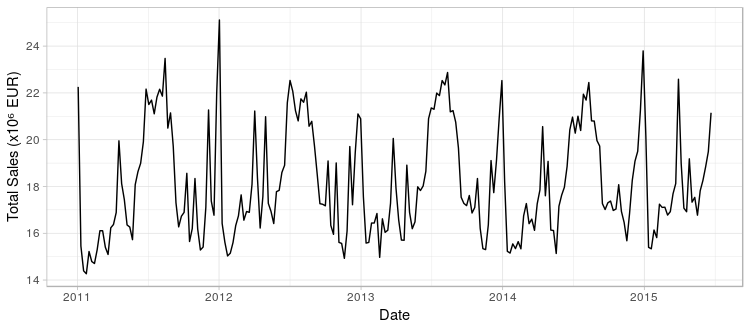
\includegraphics[scale=0.6]{figures/01_Sales.png}
\caption{Total weekly sales. Jan-2011 to Jun-2015}\label{fig:sales}
\end{figure}



The time series analyzed in this case study contains the total weekly sales of a country-wide franchise of fast food restaurants, Figure \ref{fig:sales}, covering the period January 2011 - June 2015, thus comprising 234 observations. The total weekly sales is in fact the aggregated sum from the individual sales of the whole country network of 426 franchises. Along with the sales figures, the series includes the investment levels $\{u_{it}\}$  in advertising during this period  for seven different channels \emph{viz.} \texttt{OOH} (Out-of-home, \emph{i.e.} billboards), \texttt{Radio}, \texttt{TV}, \texttt{Online}, \texttt{Search}, \texttt{Press} and \texttt{Cinema}, Figure \ref{fig:canales}, $i=1,\ldots,7$.



\begin{figure}[h]
\centering
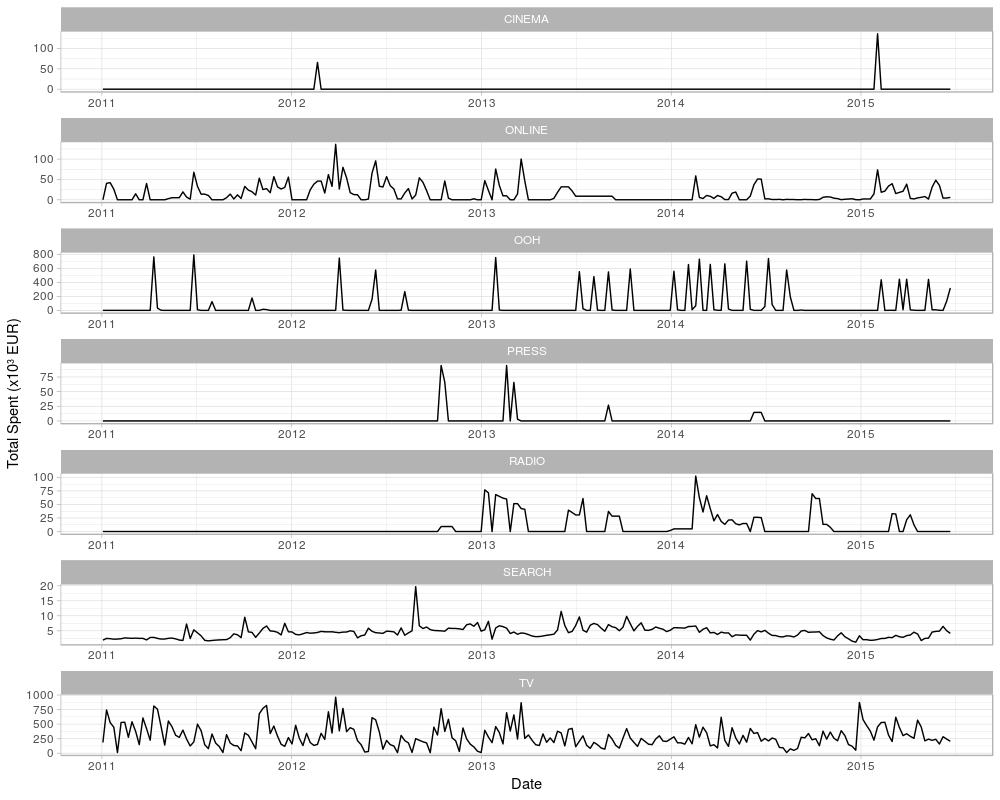
\includegraphics[scale=0.5]{figures/02_canales_b.png}
\caption{Advertising expenditure. Jan-2011-Jul-2015. \\ Note  different scales on  y-axis.}\label{fig:canales}
\end{figure}

From such graphs we observe that:
\begin{itemize}
\item In Figure \ref{fig:sales}, the series has a characteristic seasonal pattern that shows peaks in sales coinciding with Christmas, Easter and summer vacations. 
\item In Figure \ref{fig:canales} we observe that the investment levels at each channel vary largely in scale, with investments in \texttt{TV}, and \texttt{OOH} dominating the other channels.
\item The investment strategies adopted by the firm at each channel are also qualitatively different. Some of them show spikes while others depict a relatively even spread investment across time.% with many of them exhibiting pulsing behavior and regime changes, mostly attributable to the nature of the channel. 
\end{itemize}
A handful of other predictors $X_t$ which are also known to affect sales will be used in the model, all of them weekly sampled:

\begin{itemize}
\item Global economic indicators: unemployment rate (\texttt{Unemp\_IX}), price index (\texttt{Price\_IX}) and consumer confidence index (\texttt{CC\_IX}).
\item Climate data: average weekly temperature (\texttt{AVG\_Temp}) and weekly rainfall (\texttt{AVG\_Rain}) along the country.
\item Special events: holidays (\texttt{Hols}) and important sporting events (\texttt{Sport\_EV}).
\end{itemize}

\paragraph{Experimental setup.}

Following the notation in Section \ref{sec:model}, we consider three model variants for the particular dataset in increasing order of complexity:

%Baseline, Reg1, Regression2

\begin{itemize}
\item \textbf{Baseline model}, which makes use of no external variables $$Y^{\text{B}}_t = Y_{NA,t} + Y_{T, t}.$$
\item \textbf{Auto-regression}: this model  incorporates the external ambient and investment variables, so the equation of the model becomes 
\begin{equation}\label{eq:autoreg}
Y_t^{\text{RA}} = Y_{NA,t} + Y_{T, t} + Y_{R,t}.
\end{equation}
We select an expected model size\footnote{defined as the average number of selected regression features.} of 5 in the spike and slab prior, letting all variables to be treated equally.
\item \textbf{Regression (forcing)}: the model has same equation as Eq. (\ref{eq:autoreg}) (we will refer to it as \text{RF}).
%$$ Y_t^{\text{RF}} = Y_{NA,t} + Y_{T, t} + Y_{R,t}.$$ 
However, in the prior we force investment variables to be used by setting their corresponding $\pi_i = 1$, and imposing an expected model size of 5 for the rest of the variables.
\end{itemize}
In all cases, only the five principal advertising channels (\texttt{TV}, \texttt{OOH}, \texttt{ONLINE}, \texttt{SEARCH} and \texttt{RADIO}) will be used; the remaining two (\texttt{CINEMA} and \texttt{PRESS}) are sensibly lower both in magnitude and frequency than the others so we can safely disregard them in a first approximation. 


As customary in a supervised learning setting with time series data, we perform the following split of our dataset: since it comprises four years of sales, we take the first two years of observations as training set, and the rest as holdout, in which we assess several predictive performance criteria. Before fitting the data, we scale the series to have zero mean and unit variance as this increases MCMC stability. Reported sales forecasts are transformed back to the original scale for easy interpretation. The models were implemented in R  using the \texttt{bsts} package \parencite{scott2016bsts}.
% such as root mean squared error (RMSE).
%pang propone no poner el RMSE, porque no mide la calidad de nuestras predicciones de la varianza, y es mejor no meternos en berenjenales hablando de scoring rules ni las otras alternativas...

%Amongst the variants for each component discussed above, we can choose the ones that maximize the log-likelihood, or minimize some criterion like BIC or RMSE over a validation set.



\subsection{Discussion of results}

It is customary to aim at models achieving good predictive performance. %Otherwise, the proposed framework would be unusable in a real-world scenario such as the one described in the previous Section. 
For this reason, we test  our three models using two metrics:

\begin{itemize}
\item Mean Absolute Percentage Error: $$ \text{MAPE} = \frac{100\%}{T}\sum_{t=1}^T \frac{|y_t - \hat{y}_t|}{y_t},$$
where $y_t$ denotes the actual value; $\hat{y}_t$, the mean one-step-ahead prediction; and, $T$ is the length of the hold-out period.
%\item Mean Absolute Percentage Error: $$ \text{MAPE} = \frac{100\%}{T}\sum_{t=1}^T \frac{| y_t - \hat{y}_t | }{y_t} $$ 
\item Cumulative Predicted Sales over a year $Y$:
$$
\text{CPS}_{Y} = \sum_{t \in \mathcal{T}(Y)} \hat{y}_t
$$
where $\mathcal{T}(Y)$ denotes the set of time-steps $t$ contained in year $Y$.
\end{itemize}
% In addition, incorporating external information helps unbiasedness, as $\text{MPE}_{\text{RA}}$ and $\text{MPE}_{\text{RF}}$ are closer to zero than the baseline counterpart. 
These scores are reported in Table \ref{tab:mapes} with sales in million EUR. Note that the models which include external information (RA and RF) achieve better accuracy than the baseline. In addition, 
predictions are unbiased, since cumulative predictions are extremely close to their observed counterparts. Overall, we found the predictive performance of our models to be successful for a business scenario, as we achieve under 5\% relative absolute error using the variants augmented with external information. This is clearly useful for a decision maker who wants to forecast their weekly sales one week ahead to within a 5\% error in the estimation.

\begin{table}[h]
\centering
\begin{tabular}{|l|c|c|c|}
\hline
Model & MAPE & $\text{CPS}_{2013}$ & $\text{CPS}_{2014}$ \\
\hline
B &  5.85\% &   9660 & 9627 \\
RA &  4.62\% &  9680 & 9613 \\
RF &  4.59\% &  9665 & 9582 \\
\hline
\multicolumn{2}{|c|}{Cumulative True Sales:} & 9666 & 9610 \\
\hline
\end{tabular}
\caption{Accuracy measures for each model variant.} \label{tab:mapes}
\end{table}

% 966583043,  960975655

% 965992230 & 962687592 \\
% 968050055 & 961308693\\
% 966482366 & 958161307\\

Figure \ref{fig:forecasts} displays the predictive ability of model RF over the hold-out period. The model seems sufficiently flexible to adapt to fluctuations such as the peaks at Christmas. Predictive intervals also adjust their width with respect to the time to reflect varying uncertainty, yet in the worst cases they are sufficiently narrow. Further information can be tracked in Figure \ref{fig:residuals}, where mean standardized residuals are plotted for each model variant. Notice that the residuals for models RA and RF are roughly comparable, being both sensibly smaller than those of the baseline. This means that the simpler Nerlove-Arrow model benefits from the addition of the ambient variables $X_i$, as suggested in our findings from Table \ref{tab:mapes}.
%We continue, a plot of the standardized residuals of each model is depicted in \ref{fig:residuals}.
\begin{figure}[h]
\centering
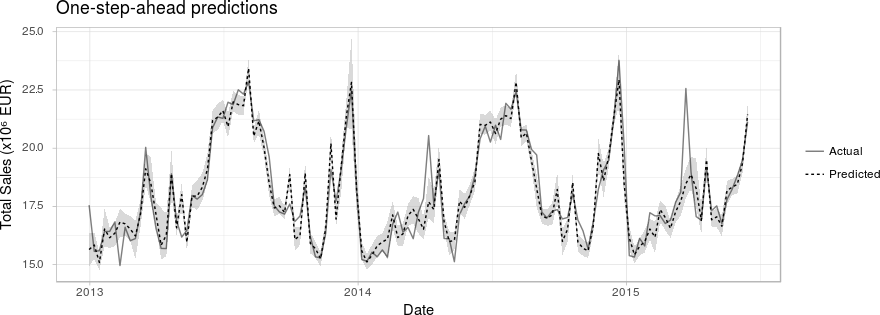
\includegraphics[scale=0.55]{figures/forecasts.png}
\caption{One-step-ahead forecasts of  RF model versus actual data during hold-out period. 95\% predictive intervals depicted in light gray.}\label{fig:forecasts}
\end{figure}



\begin{figure}[h]
\centering
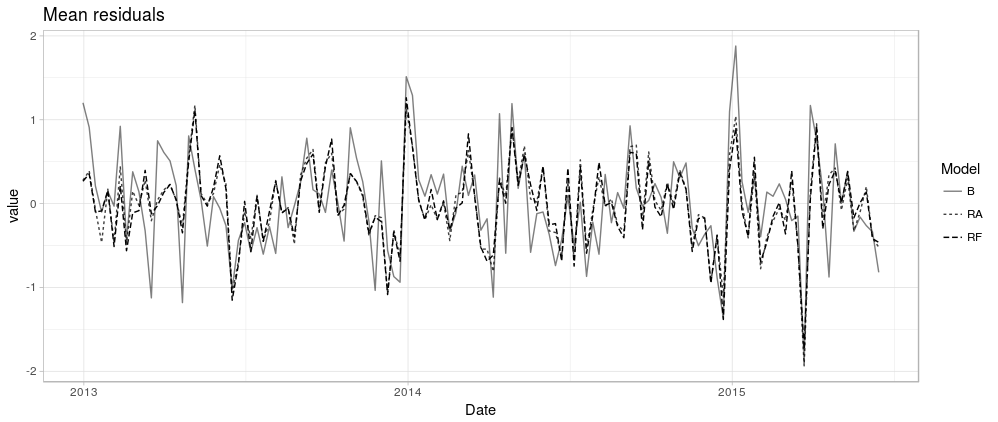
\includegraphics[scale=0.6]{figures/resis.png}
\caption{Mean residuals for each model}\label{fig:residuals}
\end{figure}

Having built good predictive models, we inspect them more closely with the aim of performing valuable inferences in our business setting. The average estimated parameter and expected standard deviations of the $q_i$ coefficients for the different advertising channels are displayed in Table \ref{tab:1}. We also show the weights of the ambient variables $X_i$ for the augmented models RA and RF in Table \ref{tab:11}, as well as the probability of a variable being selected in the MCMC simulation for a given model in Figure \ref{fig:inc_probas}. Convergence diagnostics of the MCMC scheme are reported in Appendix \ref{app:GR}.

%After we have good models, we perform summarys of coefficients. First, values \ref{tab:1} and then, inclusion probas



\begin{table}[h]
\centering
\begin{tabular}{ |l|c|c|c|c|c|c|c| }
  \hline
  & \multicolumn{2}{|c|}{Model B} & \multicolumn{2}{|c|}{Model RA} & \multicolumn{2}{|c|}{Model RF}\\
  \hline
  Channel & mean & sd & mean & sd & mean & sd\\
  \hline
  \texttt{y\_AR} & \textbf{8.00e-01} & \textbf{5.10e-02} &  \textbf{5.17e-01} &  \textbf{4.50e-02} &  \textbf{5.07e-01} &  \textbf{4.55e-02}   \\
  \texttt{OOH} & 9.30e-03 & 3.11e-02 & 1.15e-03 & 9.54e-03  & \textbf{6.10e-02} &  \textbf{3.54e-02}\\
  \texttt{ONLINE} & 1.10e-03 & 9.25e-03  & 1.95e-03 &  1.23e-02 & \textbf{9.04e-02} & \textbf{4.01e-02}\\
  \texttt{RADIO} & -5.34e-04 & 6.80e-03  &-2.61e-05 & 2.30e-03 &   -2.57e-02 & 3.42e-02\\
  \texttt{TV} & -2.85e-04 & 5.12e-03 & -5.53e-05 & 3.71e-03  & -6.14e-02 & 4.21e-02\\
  \texttt{SEARCH} & 1.51e-05  & 2.74e-03  & 8.58e-05 & 2.49e-03  & 1.38e-02 & 3.50e-02 \\
    \hline
\end{tabular} \caption{Expected value and standard error of  $q_i$. Statistically significant coefficients  in bold.}\label{tab:1}
\end{table}

\begin{table}[h]
\centering
\begin{tabular}{ |l|c|c|c|c|c| }
  \hline
  &  \multicolumn{2}{|c|}{Model RA} & \multicolumn{2}{|c|}{Model RF}\\
  \hline
  Channel & mean & sd & mean & sd\\
  \hline
  \texttt{Sport\_EV} & \textbf{-2.06e-01} & \textbf{3.80e-02} & \textbf{-2.00e-01} &\textbf{ 3.71e-02} \\
  \texttt{AVG\_Temp} &  \textbf{2.57e-01} & \textbf{4.43e-02} & \textbf{2.43e-01} & \textbf{4.65e-02}   \\
  \texttt{Hols} & \textbf{3.10e-01} &\textbf{ 3.70e-02}   & \textbf{3.15e-01} & \textbf{3.72e-02}  \\
  \texttt{AVG\_Rain} &  -2.86e-02 & 5.01e-02 & -1.96e-02 & 4.14e-02     \\
  \texttt{Price\_IX} &  1.38e-03 &  1.15e-02 & 3.60e-03 & 1.92e-02  \\
  \texttt{Unemp\_IX} &  6.34e-05 & 3.32e-03 & 2.36e-04 & 7.79e-03  \\
  \texttt{CC\_IX} & 6.27e-07 & 2.94e-03 & 2.85e-04 & 5.50e-03 \\
    \hline
\end{tabular} \caption{Expected value and standard error of  $\beta_i$. Statistically significant coefficients in  bold.}\label{tab:11}
\end{table}


% Mover tablas debajo, aunque primero grafica del error.

\begin{figure}[h]
\centering
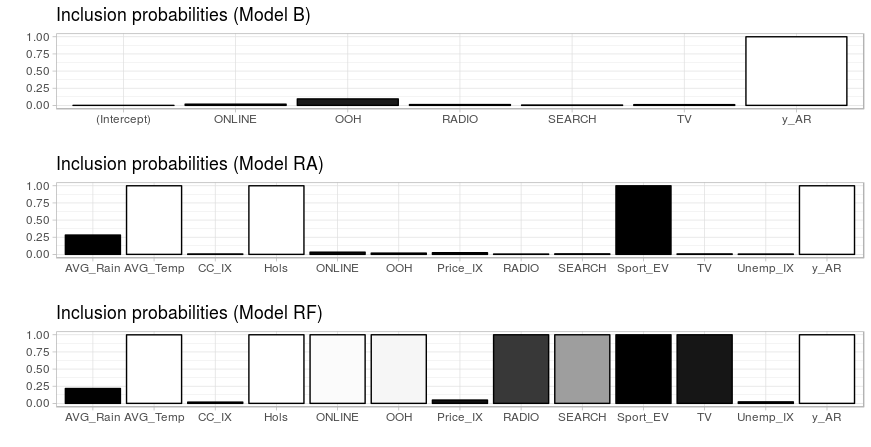
\includegraphics[scale=0.6]{figures/inc_probas2.png}
\caption{Selection probabilities in  MCMC simulation for each predictor variable in the  models. Color code shows variables positively (white) or negatively (black) correlated with sales. }\label{fig:inc_probas}
\end{figure}

%\begin{figure}[h]
%\centering
%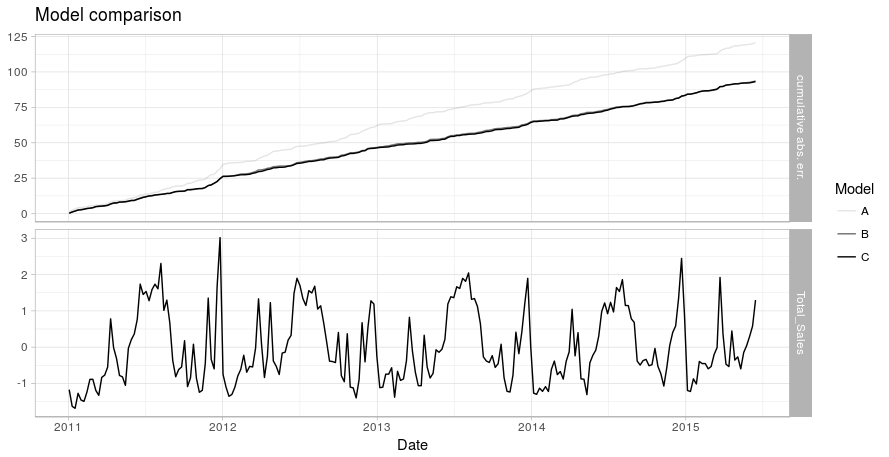
\includegraphics[scale=0.65]{figures/comparison.pdf}
%\caption{Cumulative absolute one step ahead prediction errors for each model}\label{fig:comparison}
%\end{figure}

Looking at the ambient variables, the following comments seem in order:
\begin{itemize}
%\item The one-step prediction error for models $2$ and $3$ is roughly equal, being both sensibly lower than that of model $1$. This means that the simpler Nerlove-Arrow model is biased and profits from the addition of the ambient variables $X_i$.

\item From Table \ref{tab:11} we see that the socio-economic indicators (unemployment rate, inflation and consumer confidence) do not seem statistically relevant for this problem. 

\item Looking at the sign of the coefficients of the most significant regressors $X_i$ (\texttt{Hols}, \texttt{Sport\_EV}, \texttt{AVG\_Temp} and \texttt{AVG\_Rain}) we see that they are as we would naturally expect. Moreover, their absolute value is well above the error in both models RA and RF, a strong indicator of their influence in the expected weekly sales (\emph{cf.} Table \ref{tab:11}, Figure \ref{fig:inc_probas}). 

\item We see, for instance, that sporting events are negatively correlated with sales. This can be interpreted as follows: major sporting events in the country where the data have been recorded receive a large media coverage and are followed by a significant fraction of the population. The restaurant chain in this study has no TVs broadcasting in their restaurants, so customers probably choose alternative places to spend their time on a day when \texttt{Sport\_EV} = 1. 

\item The sign of \texttt{Hols} and $\texttt{AVG\_Temp}$ is positive, showing strong evidence for the fact that sales increase in periods of the year where potential customers have more leisure time, like national holidays or  summer vacation. 

\item One would expect \texttt{AVG\_Rain} to be negatively correlated with restaurant sales, but in our study (despite having negative sign) it is not statistically significant. A possible explanation is that \texttt{AVG\_Rain} records average rainfall over a large country. %A more fine-grained analysis on a restaurant by restaurant basis incorporating local weather conditions will be performed in a future study, probably revealing a larger influence of this variable on the sales prediction.

\end{itemize}

Next, we turn our attention to the investment variables across different advertising channels.

\begin{itemize}

\item The advertising channels $u_i$ are almost never selected in model RA, and their $q_i$ coefficients are not significantly higher than their errors to be considered influential in the model. In model RF, however, there is strong evidence that their effect is more than a random fluctuation (\emph{cf.} Table \ref{tab:1}, Figure \ref{fig:inc_probas}). 
\item The negative sign in both \texttt{RADIO} and \texttt{TV} in all three models suggests that (at least locally) part of the expenditures in these two channels should be diverted towards other channels with positive sign on their $q_i$ coefficients, specially to the channel with the strongest positive coefficient (\texttt{ONLINE} and \texttt{OOH}).
\item It is interesting that the trend that shows the year-to-year advertising budget of this firm (\emph{cf.} figure \ref{fig:yearly}) has a significant reduction in \texttt{TV} expenditures and a big increase in \texttt{OOH}. \texttt{RADIO} however is not reduced accordingly but increased, and \texttt{ONLINE} ---\,which our model considers the best local inversion alternative\,--- follows the inverse path\footnote{It has to be noted, however, that \texttt{ONLINE} expenditures are typically correlated with discounts, coupons and offers, and this information was not available to us.}.
\item The autoregressive term is close to $0.5$, which means that the immediate effect of advertising is roughly half to the \textit{long run accumulated effects}.
%\item Despite modelling the noise term with student's $t$ disturbances, the residual plots still show strong fluctuations which influence heavily the model's absolute error.
\end{itemize}


\begin{figure}[h]
\centering
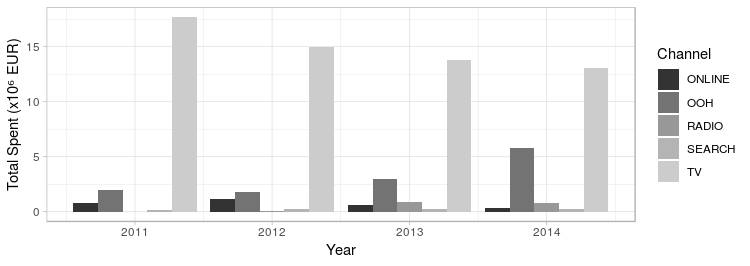
\includegraphics[scale=0.75]{figures/anuales}
\caption{Yearly total expenditures on advertising campaigns for the restaurant chain, per advertising channel.}\label{fig:yearly}
\end{figure}






%\subsubsection{Model comparison}

%Comparison of models: no regressors; linear relationships; black-box model (cumulative absolute error)

\paragraph{Budget allocation. Model-based solutions.}\label{section: budget allocation}

Based on the above, we propose a model which can be used as a decision support system for the manager, helping her in adopting the  investment strategy in advertising. The company is interested in maximizing the expected sales for the next period, subject to a budget constraint for the advertising channels and also a risk constraint, i.e., the variance of the predicted sales must be under a certain threshold.
This optimization problem based on one-step-ahead forecasts can be formulated as a non linear, but convex, problem that depends on  parameter $\sigma^2$:

\begin{equation*}
\begin{aligned}
& \underset{u_{(t+1),1}...u_{(t+1),k}}{\text{maximize}}
& &  E[ \bar{y}_{t+1} | y_{1:t}, x_{t+1}, u_{t+1}] \\
& \text{subject to}
& & \sum_{i=1}^k  u_{(t+1),i} \leq b_{t+1} \\
& & & Var[ \bar{y}_{t+1} | y_{1:t}, x_{t+1}, u_{t+1}] \leq \sigma^2, \\
\end{aligned}
\end{equation*}
where $b_t$ is the total advertising budget for week $t$ and $\sigma$ is a parameter that controls the risk of the sales. We have made explicit the dependence on the regressor variables $x_t$ and advertisement investments $u_t$ in the mean and variance expressions.
Solving for different values of $\sigma$, we obtain a continuum of Pareto optimal investment strategies that we can present to the manager, each one representing a different trade-off between risk and expected sales that we can plot in a risk-return diagram.
This approach greatly reduces the decision space for the manager.

A possible alternative would be to rewrite the objective function as 
$$E[ \bar{y}_{t+1} | y_{1:t}, x_{t+1}, u_{t+1}] - \lambda \sqrt{Var[ \bar{y}_{t+1} | y_{1:t}, x_{t+1}, u_{t+1}]}$$ 
which may be regarded as a lower quantile if the predictive samples $\bar{y}^{(i)}_{t+1}$ are normally distributed.
As in the previous approach, different values of $\lambda$ represent different risk-return trade-offs.

If the errors in the observation equation (\ref{eq:obs}) are Normal, the computations for expected predicted sales and the above variance can be done exactly and quickly using conjugacy as in \parencite[3.7.1]{zbMATH06123712}.
Otherwise, the desired quantities can be computed through Monte Carlo simulation, as in Section \ref{s:MCMC}.

Note that due to the nature of the state-space model, it is straightforward to extend the previous optimization problem over $k$ timesteps, for $k>1$.
The two objectives would be the expected total sales and the total risk over the period $t+1,\dots,t+k$.
For normally distributed errors, the predicted sales on the period also follow a Normal distribution, which makes computations specially simple.

The above optimization problem may not need to be solved by exhaustively searching over the space of possible channel investments. In a typical business setting, the manager would consider a discrete set of $S$ investment strategies that are easy to interpret, so she may perform $S$ simulations of the predictive distribution and use the above strategy to discard the Pareto suboptimal strategies.

\subsection{Discussion}

TODO

\iffalse
\subsection{Large scale approaches to Bayesian inference in DLMs}

\begin{itemize}
    \item Describre Sarkka recent parallel algorithm for Kalman filter.
    \item Plot graphics for synthetic datasets of time vs number of points, comparing sequential vs parallel Kalman filter.
    \item Propose algorithm for generalizing to Bayesian inference in full DLMs, of form $p(x_{1:T}, z_{1:T}| \theta)$, where $x_{1:T}$ are the observations, $z_{1:T}$ the state variables and $\theta$ a parameter of interest.
    \begin{enumerate}
    \item Compute marginal likelihood $p(x_{1:T}|\theta)$ using the Parallel Kalman filter to marginalize out the state variables.
    \item Iterate for one step using any SG-MCMC method to obtain posterior samples of the parameter, e.g., 
    $$
    \theta_{t+1} = \theta_t + \eta\nabla \log p(x_{1:T}|\theta_t) + \mathcal{N}(0, 2\eta I)
    $$
    \end{enumerate}
    
    Both steps are scalable to large data regimes, and we could alternate them until some convergence criteria is satisfied
    \item Apply it to the McDonalds data, compare times.
\end{itemize}
\fi

\section{Current challenges: deep models and big data}

\subsection{Introduction}

The history of neural network (NN) models have gone 
through several waves of popularity. The first 
one starts with the introduction of the perceptron
by \textcite{rosenblatt1958perceptron} and its training algorithm 
for classification in linearly separable problems.
Limitations brought up by 
\textcite{minsky} somehow reduced the enthusiasm
about these models by the early 70's.
The next period of success coincides with the emergence
of results presenting NNs as universal
approximators, e.g.\ \parencite{cybenko1989approximation}. Yet 
technical issues and the emergence of other paradigms like 
support vector machines led, essentially,
to a new stalmate by the early 2000's. Finally, several of the 
technical issues were solved, coinciding with the 
availability of faster computational tools,
improved algorithms and the emergence of
large annotated datasets. These produced outstanding 
applied developments leading, over the last decade, to the current boom 
surrounding deep NNs \parencite{10.5555/3086952}. 

This section overviews  
recent advances in NNs. 
There are numerous reviews with various emphasis 
including physical \parencite{cirac}, computational \parencite{chollet}, mathematical \parencite{maths} and pedagogical \parencite{teach} pùrposes, 
notwithstanding  those concerning different  application areas, 
from autonomous driving systems (ADS) \parencite{rumanos} to
drug design \parencite{hessler}, to name but a few. 
Our emphasis is on statistical
aspects and, more specifically, on Bayesian approaches
to NN models for reasons that will become 
apparent during this thesis but include mainly:
the provision of improved uncertainty estimates, which is
of special relevance in decision support under uncertainty; their 
increased generalization capabilities; their 
enhanced robustness against adversarial attacks; 
their improved capabilities for model calibration;
and the possibility of using sparsity-inducing priors
to promote simpler NN architectures.

We first recall basic results from (the now-called) 
shallow NNs.
Section \ref{sec:dnn_examples} then covers deep NNs, including their most
relevant 
variants, as well as classical and Bayesian approaches
for their analysis. Next, Section \ref{sec:dnn_examples}
presents two examples illustrating
diverse NN architectures.

%%%%%%%%%%%%%%%%%%%%%%%%%%%%%%%%%%%%%%%%%
\subsection{Shallow neural networks}
This section briefly introduces key concepts
about shallow networks to support later discussions on current approaches.
Our focus will be mainly on nonlinear regression 
problems. Specifically, we aim at approximating 
an $r$-variate response (output) $y$ with respect to $p$ explanatory 
(input) variables $x=(x_1,\ldots,x_p)$ through the 
model
\begin{eqnarray}\label{kantora}
  y         & = & \sum_{j=1}^m \beta_j \psi(x' \gamma_j) +
                    \epsilon %_i,~~i=1,\ldots,n
                    \nonumber\\
              & & \epsilon \sim N(0,\sigma^2),
                  \nonumber \\
              & & \psi(\eta) = \exp(\eta)/(1+\exp(\eta)).
                  \end{eqnarray}
This defines a neural network with one hidden 
layer with $m$ hidden neurons and logistic 
activation functions.
Figure \ref{figuradkk1} sketches 
a graphical model of a shallow NN with 10 inputs, 4 hidden nodes and 
2 outputs. 
\begin{figure}
    \centering
    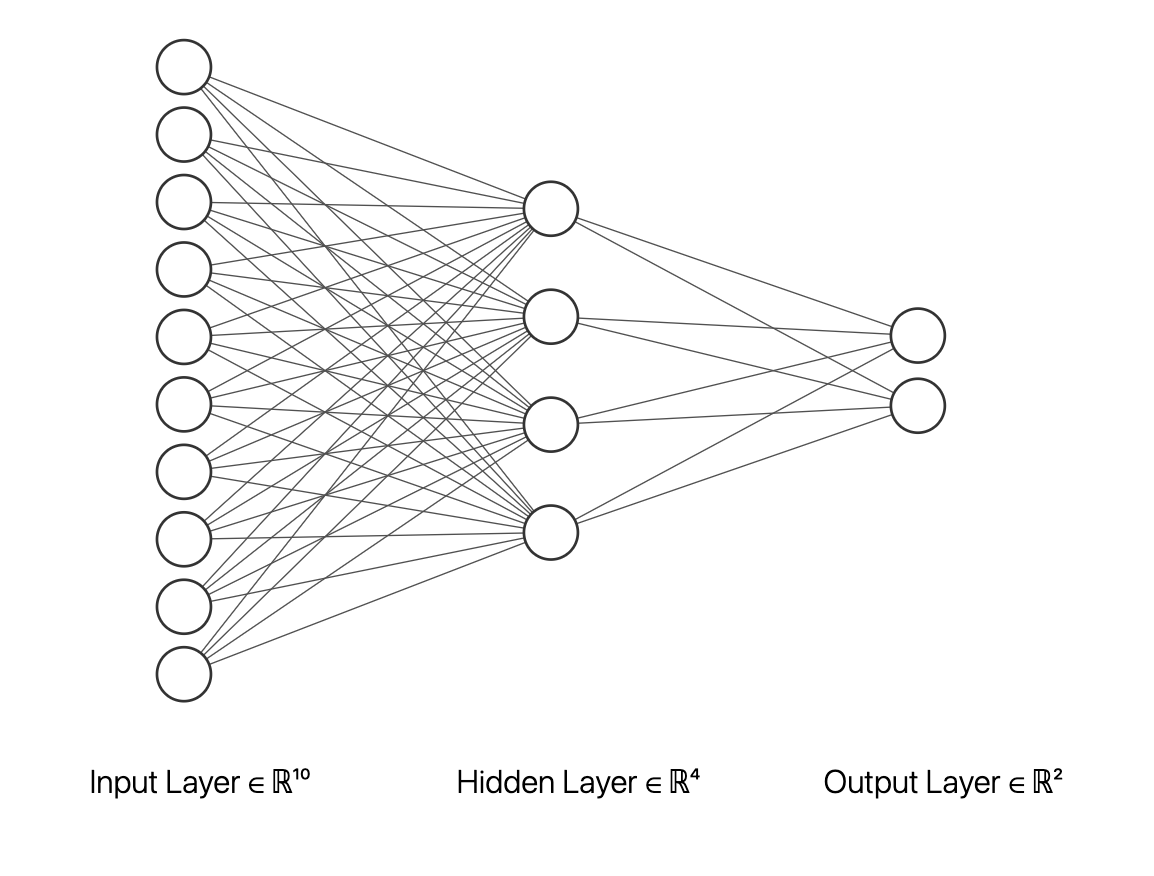
\includegraphics[scale=0.5]{figures/net1.png}
    \caption{A shallow NN architecture with 4 hidden nodes and 2 scalar outputs}
    \label{figuradkk1}
\end{figure}

Let us designate with $\beta=(\beta_1,\ldots,\beta_m)$ and $\gamma=(\gamma_1,\ldots,\gamma_m)$ the network parameters. $\sigma$  
will be considered a hyperparameter. Clearly, the model
is linear in $\beta$ but non-linear in  
$\gamma$. Interest in this type of models stems from 
results such as those of \textcite{cybenko1989approximation}
who presents them as universal approximators:
 any continuous function in the 
$r$-dimensional unit cube 
may be approximated by models of type
$\sum_{j=1}^m \beta_j \psi(x' \gamma_j)$
when the $\psi$
functions are sigmoidal (as with the logistic) and
$m\rightarrow \infty$. Our discussion focuses on $r=1$.



%%%%%%%%%%%%%%%%%%%%%%%%%%%%%%%%%%%%%%%
\paragraph{Classical approaches.}\label{sanchez}

Given $n$ observations $D=\{ (x_i, y_i), i=1,...,n \}$,
 maximum likelihood estimation (MLE) 
 computes the log-likelihood and maximises it 
leading to the classical non-linear least squares problem
\begin{equation}\label{pdt}
 \min_{\beta , \gamma } f (\beta , \gamma) = \sum _{i=1}^n f_i(\beta, \gamma)  =\sum _{i=1}^n \left( y_i -
  \sum_{j=1}^m \beta_j \psi(x_i'\gamma_j) \right)^2 
 \end{equation}

\noindent Quite early, researchers paid attention to the introduction of regularisers, such as weight decay $\ell_2$ penalization \parencite{krogh1992simple}, so as to improve model 
generalization, leading to the modified optimisation problem
\begin{equation}\label{kkdbak}
 \min  g(\beta ,\gamma) = f (\beta ,\gamma ) +
 h (\beta ,\gamma ), \end{equation}
where $h(\beta , \gamma )$ represents the regularisation 
term. For example, in the above mentioned case, the 
additional term is  
$h(\beta , \gamma )= \lambda _1 \sum \beta_i ^2 +
\lambda _2 \sum \sum \gamma _{ji} ^2$. 

Typically problems (\ref{pdt}) and (\ref{kkdbak}) are solved via steepest gradient descent \parencite{meza} through iterations of the type
\[
   (\beta, \gamma )_{k+1}=
   (\beta, \gamma )_{k}- \eta \nabla g (  (\beta, \gamma )_{k} ),
   \]
where $\eta $ is frequently chosen as a fixed small learning rate parameter and $\nabla g $ is the gradient of function $g$, with respect to 
$(\beta ,\gamma )$. 


\noindent    Very importantly,  the structure of the network and the 
    chain rule of calculus %take advantage of the 
    %above structure to 
    facilitates efficient estimation of the gradients 
    via backpropagation, e.g. \parencite{rumelhart1986learning}.
    
    A problem entailed by NN model estimation is the highly multimodal nature of
    the log-likelihood for three reasons:
    invariance with respect to arbitrary relabeling of
    parameters (these may
    be handled by means of order 
    constraints among the 
    parameters);
    that inherently due to non-linearity; and, finally, 
    node duplicity (which may be dealt 
    with a model reflecting uncertainty 
    about the number of nodes,
    as explained below).
A way to mitigate multimodality is to use a global optimization method, like multistart, but
this is very demanding computationally in this domain.

Finally, note that the same kind of NN models 
may be used for nonlinear auto-regressions in
time series analysis \parencite{menchero} and 
non-parametric 
regression \parencite{insuamuller}. Moreover,
similar models may be used for classification purposes,
although this 
 requires modifying the likelihood
\\parencite{bishop2006pattern} to e.g.\
\begin{equation}
    p(y | x, \beta, \gamma) = Mult(n=1, 
    p_1 (x, \beta, \gamma) , \ldots, p_K (x, \beta, \gamma) ),
\end{equation}
that is, a draw from a multinomial distribution with $K$ classes. 
Class probabilities
 can be computed using the softmax function,
$$
p_k = \frac{\exp{\beta_k \psi(x'\gamma_k)}}{\exp{\sum_{k=1}^K \beta_k \psi(x'\gamma_k)}}.
$$


%%%%%%%%%%%%%%%%%%%%%%%%%%%%%%%%%
\paragraph{Bayesian approaches.}\label{bayeshallow}
We discuss now Bayesian approaches to shallow NNs.
assuming standard priors 
in Bayesian hierarchical modeling, see e.g.\ \textcite{LavineWest}: 
$  \beta_i      \sim  N(\mu_\beta,\sigma_\beta^2)$
and 
  $\gamma_i     \sim  N(\mu_\gamma,S_\gamma^2)$,
  completed with priors over the hyperparameters
$\mu_\beta \sim N(a_\beta,A_\beta)$,
$\mu_\gamma \sim N(a_\gamma,A_\gamma)$,
$\sigma^{-2}_\beta \sim Gamma(c_b/2,c_b/2)$,
$S_\gamma^{-1} \sim Wish(c_\gamma,(c_\gamma C_\gamma)^{-1})$ and
$\sigma^{-2} \sim Gamma(s/2, s/2)$.
In this model, 
an informative prior probability model
is meaningful as parameters are interpretable. For example, the $\beta_ j$’s would reflect the
order of magnitude of the data $y_i$; typically positive and negative values for
$\beta _j$ would be equally likely, calling for a symmetric prior around 
0 with
a standard deviation reflecting the range of plausible values for $y_i$. Similarly,
a range of reasonable values for the logistic coefficients $\gamma_ j$ will be determined
%by the meaning of the data $y_i$ being modeled,
mainly to address smoothness
issues.

Initial attempts to perform Bayesian analysis
of NNs, adopted
arguments based on the asymptotic normality of the posterior, 
as in  
\parencite{mckay} and \parencite{buntineweigend}. However these methods
fail if they are dominated by  
less important modes. %; moreover, some of the 
%hypothesis underlying asymptotics are doubtful 
%in the NN context.
 \parencite{buntineweigend} mitigate this by finding several modes and
basing inference on weighted mixtures of the corresponding normal approximations, but we return to the same issue as some
important local modes might have been left out. An alternative view was argued
by \parencite{mckay}: inference from such schemes is 
 considered as approximate
posterior inference in a submodel defined by constraining the
parameters to a neighborhood of the particular local mode. Depending on
the emphasis of the analysis, this might be reasonable, especially if in a final
implementation our aim is to set the parameters at specific values,
the usual scenario in deep learning. We prefer
though to propagate the uncertainty in parameters, since this allows
better predictions, e.g. \parencite{raftery}. 

For this, an efficient 
Markov chain Monte Carlo (MCMC) scheme
may be used \parencite{muller1998issues}. It 
 samples from the posterior conditionals when available (steps 3, 9), and use
Metropolis steps (4-8), otherwise. To fight potential inefficiencies due to
multimodality, two features are built in 
 for
fast and effective mixing over local posterior modes:
whenever
possible, the $\gamma$ weights are 
partially marginalized; second,
these weights are resampled jointly.
The key observation is that,
given
 $\gamma $,
we actually have a standard hierarchical normal linear
model \parencite{french}. This facilitates sampling from the posterior marginals of the $\beta $ weights (step 3)
 and hyperparameters (step 9) and 
 allows marginalizing the model with respect
 to the $\beta$'s
  to obtain the marginal likelihood $p(D|\gamma, \nu)$
  (step 3), where $\nu=(\mu_\beta,\sigma_\beta,\mu_\gamma,S_\gamma,\sigma^2)$ designates the hyperparameters.
The procedure runs like the described in Algorithm \ref{alg:mcmc}.

\iffalse
{\tt 
\begin{enumerate}
  \item  Start with arbitrary $(\beta , \gamma ,\nu )$.\\
    Until convergence, iterate through 2-4
  \item  Given current $(\gamma,\nu)$, draw  
    $\beta$ from  
    $p(\beta|\gamma,\nu,y)$ (a multivariate normal).
    \item  For $j=1,...,m$,
    marginalizing in $\beta$ and given $\nu$, draw $\gamma_j$ through: \\
    Generate a candidate $\tilde\gamma_j \sim g_j(\gamma_j)$. \\
    Compute 
    $
       a(\gamma_j,\tilde\gamma_j) =
       \min\left(1,\frac{p(D |\tilde\gamma,\nu)}
                       {p(D |\gamma,\nu)}\right)
    $
    with $\tilde\gamma = (\gamma_1,\gamma_2,\ldots,\tilde\gamma_i, ...,\gamma_m)$.\\
    With probability $a(\gamma_j,\tilde\gamma_j)$ replace $\gamma_j$
    by $\tilde\gamma_j$. If not, preserve $\gamma_j$.
      \item Given $\beta$ and $\gamma$, replace $\nu$
        based on their posterior conditionals:\\
 $p(\mu_\beta|\beta,\sigma_\beta)$ is normal;
 $p(\mu_\gamma|\gamma,S_\gamma)$, multivariate normal;
 $p(\sigma_\beta^{-2}|\beta,\mu_\beta)$, Gamma; 
    $p(S_\gamma^{-1}|\gamma,\mu_\gamma)$, Wishart; 
    $p(\sigma^{-2}|\beta,\gamma,y)$, Gamma.
    \end{enumerate}
}
\fi

\begin{algorithm}[!ht]
\begin{algorithmic}[1]
\State Start with arbitrary $(\beta , \gamma ,\nu )$.
\While{not convergence} 
 \State Given current $(\gamma,\nu)$, draw  
    $\beta$ from  
    $p(\beta|\gamma,\nu,y)$ (a multivariate normal).
    \For{$j=1,...,m$, marginalizing in $\beta$ and given $\nu$ } 
    \State Generate a candidate $\tilde\gamma_j \sim g_j(\gamma_j)$.
    \State Compute 
    $
       a(\gamma_j,\tilde\gamma_j) =
       \min\left(1,\frac{p(D |\tilde\gamma,\nu)}
                       {p(D |\gamma,\nu)}\right)
    $
    with $\tilde\gamma = (\gamma_1,\gamma_2,\ldots,\tilde\gamma_i, ...,\gamma_m)$.
    \State With probability $a(\gamma_j,\tilde\gamma_j)$ replace $\gamma_j$
    by $\tilde\gamma_j$. If not, preserve $\gamma_j$.
    \EndFor
    \State Given $\beta$ and $\gamma$, replace $\nu$
        based on their posterior conditionals:
 $p(\mu_\beta|\beta,\sigma_\beta)$ is normal;
 $p(\mu_\gamma|\gamma,S_\gamma)$, multivariate normal;
 $p(\sigma_\beta^{-2}|\beta,\mu_\beta)$, Gamma; 
    $p(S_\gamma^{-1}|\gamma,\mu_\gamma)$, Wishart; 
    $p(\sigma^{-2}|\beta,\gamma,y)$, Gamma.
    
\EndWhile
\end{algorithmic}
 \caption{MCMC sampler}\label{alg:mcmc}
\end{algorithm}



\noindent For proposal generation distributions $g_j(\cdot)$,
normal multivariate distributions
$N(\gamma_j,c^2 C_\gamma)$ are 
adopted. % with $c=0.1$ work in
%applications. 
Appropriate values for $c$ can be found by trying
a few alternative choices until acceptance rates around
 0.25 are achieved \parencite{gamerman}. 

Combined with model augmentation to a variable architecture,
 this leads to a useful scheme
for complete shallow NN analyses as it allows for 
the identification of
architectures supported by data, by  
contemplating $m$ as an additional parameter.
A random $m$ with a prior 
favoring smaller values reduces posterior multimodality.
Moreover, as marginalization over $\gamma_ j$ requires inversion of matrices
of dimension related to $m$, 
avoiding unnecessarily large
hidden layers is critical to
mitigating computational effort.
 Thus, we assume 
a maximum size $m^*$ for the network and introduce 
indicators  $d_j$ suggesting whether node
$j$ is included ($d_j=1$) or not ($d_j=0$). 
We  also 
include a linear regression term $x'a$
to favor parsimony. On the whole, the model
becomes 
\begin{eqnarray*}
  y          & = & x_i'a + \sum_{j=1}^{m^*} d_j\beta_j \psi(x '\gamma_j) +
                    \epsilon \\ %_i,i=1,...,N\nonumber\\
                    & & \epsilon \sim N(0,\sigma^2),\nonumber \\
                    & &    \psi(\eta) = \exp(\eta)/(1+\exp(\eta)),
                        \nonumber \\
  Pr(d_j=0|d_{j-1}=1)   & = & 1-\alpha, \nonumber\\
  Pr(d_j=1|d_{j-1}=1)   & = & \alpha, \nonumber\\
  \beta_i    \sim  N(\mu_b,\sigma_\beta^2),& 
  a     \sim  N(\mu_a,\sigma_a^2), &   \gamma_i   \sim  N(\mu_\gamma,\Sigma_\gamma).
                \label{eq:model-var}
\end{eqnarray*}
Learning is done through a reversible jump sampler
\parencite{green} embedding our first algorithm.
As a consequence, we perform inference
about the architecture based on the distribution of 
 $p(m|D)$. 

 \textcite{neal2012bayesian} proposed using an 
algorithm merging conventional Metropolis-Hastings chains with sampling
techniques based on dynamic simulation, the currently popular
Hamiltonian Monte Carlo (HMC) approaches.
Let us designate by $\theta$ the NN 
weights, $\theta = (\beta, \gamma)$, and denote the potential energy function as
$$
U(\theta) = \tau_{\beta}\sum_{i=1}^m \beta_i^2/2 + \tau_{\gamma} \sum_{i=1}^m \gamma_i^2/2 + \tau \sum_{j=1}^n (y_j - f(x_i, \theta_i))^2/2,
$$
where $\tau_{\beta}, \tau_{\gamma}, \tau$ are hyperparameters 
controlling regularization, similarly to (\ref{kkdbak}). 
Let us also introduce the hamiltonian 
$$
H(\theta, r) = U(\theta) + \frac{1}{2} \sum_{i=1}^m r_i^2,
$$
with momentum variables $r$ of the same dimension as $\theta$; such 
 variables serve to accelerate the walk towards posterior modes. Then, the HMC scheme would be as described in Algorithm \ref{alg:hmc}.

\iffalse
{\tt 
\begin{enumerate}
  \item  Start with arbitrary $\theta_0 = (\beta _0, \gamma _0)$.\\
    Until convergence, iterate through 2-4
  \item  Given current $\theta_t$ and $r_t \sim \mathcal{N}(0, I)$, perform $T$ leapfrog integration
  steps 
  \begin{align*}
  r_{t + \frac{\epsilon}{2}} &= r_t - \frac{\epsilon}{2}\nabla U(\theta_t) \\
   \theta_{t+ \epsilon} &= \theta_t + \epsilon  r_{t + \frac{\epsilon}{2}} \\
   r_{t + \epsilon} &= r_{t + \frac{\epsilon}{2}} - \frac{\epsilon}{2}\nabla U(\theta_{t+ \epsilon})
    \end{align*}
    to reach  $\theta^*$ and $r^*$. % be the final solution 
    %and its corresponding momentum.
\item Compute $\alpha(\theta_t, \theta^*) = \min \left\{ 1, \frac{\exp H(\theta^*, r^*)}{\exp H(\theta_0, r_0)} \right\} $
\item Accept $\theta^*$ with probability $\alpha(\theta_t, \theta^*)$, else discard it.
    \end{enumerate}
}
\fi


\begin{algorithm}[!ht]
\begin{algorithmic}[1]
\State Start with arbitrary $\theta_0 = (\beta _0, \gamma _0)$.
\While{not convergence}
  \State Given current $\theta_t$ and $r_t \sim \mathcal{N}(0, I)$, perform one or more leapfrog integration
  steps 
  \begin{align*}
  r_{t + \frac{1}{2}} &= r_t - \frac{\epsilon}{2}\nabla U(\theta_t) \\
   \theta_{t+ 1} &= \theta_t + \epsilon  r_{t + \frac{1}{2}} \\
   r_{t + 1} &= r_{t + \frac{1}{2}} - \frac{\epsilon}{2}\nabla U(\theta_{t+ 1})
    \end{align*}
    to reach  $\theta^*$ and $r^*$.
    \State Compute $\alpha(\theta_t, \theta^*) = \min \left\{ 1, \frac{\exp H(\theta^*, r^*)}{\exp H(\theta_t, r_t)} \right\} $.
   \State Accept $\theta^*$ as $\theta_{t+1}$ with probability $\alpha(\theta_t, \theta^*)$, else discard it. 
  
 \EndWhile
 \end{algorithmic}
 \caption{HMC sampler}\label{alg:hmc}
\end{algorithm}





%%%%%%%%%%%%%%%%%%%%%%%%%%%%%%%%%%%%%%%%
\subsection{Deep neural networks}\label{sec:dnn_examples}

Training by backpropagation has been in use 
for many years by now.
The decade of the 2010's saw major developments
leading to 
the boom around deep learning \parencite{10.5555/3086952}
or inference and prediction with deep NNs. 
Such advances include:
the availability of fast GPU kernels and routines
facilitating much faster training;
the access to massive amounts of data (e.g.\ Imagenet), which prevented overfitting to smaller datasets; 
the creation of new architectures, which prevented  convergence issues, such as the vanishing gradient problem; 
and, finally, the provision of automatic differentiation libraries such as Tensorflow, Caffe or Theano.
Figure \ref{figuradkk} displays an example
of what are now designated 
deep NNs, that is NNs with more than one hidden
layer, four in the portrayed case.
\begin{figure}
    \centering
    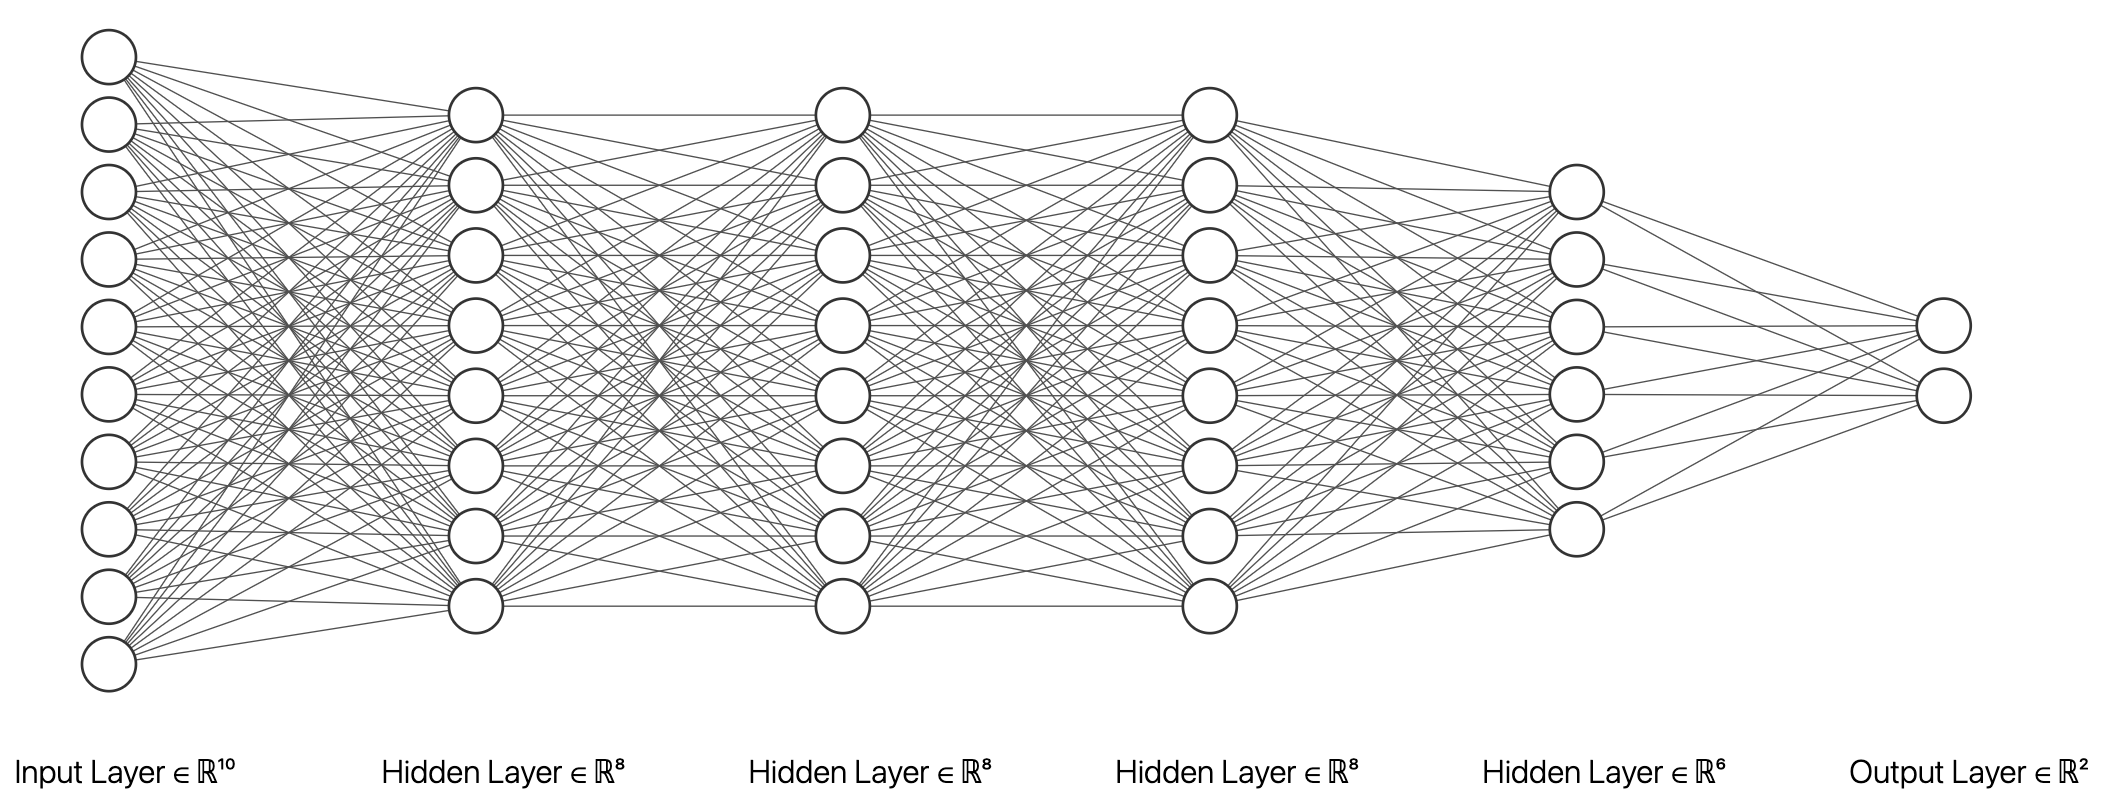
\includegraphics[scale=0.35]{figures/net2.png}
    \caption{A deep NN architecture with four hidden layers and 2 scalar outputs}
    \label{figuradkk}
\end{figure}


A deep NN may be defined through   
a sequence of functions $\lbrace f_0, f_1, ..., f_{L-1} \rbrace$, each parametrized by some weights $\gamma_l$
of dimension $m_l$  (the corresponding number of hidden nodes) with the output of each layer being the input of the following one, as in
$$
    z_{l+1} = f_l ( z_l, \gamma_l).
$$
Lastly, we compute a prediction from the hidden activations of the last layer, as in Eq. (\ref{kantora})
\begin{eqnarray}
y         & = & \sum_{j=1}^{m_L} \beta_j z_{L,j} +
                    \epsilon %_i,~~i=1,\ldots,n
                    \nonumber\\
              & & \epsilon \sim N(0,\sigma^2),
                  \nonumber \\
\end{eqnarray}

Modern architectures do not longer require the
$f_l$ functions to be sigmoidal (like the  
logistic functions in (\ref{kantora})) and include  
the rectified linear unit (ReLU), the leaky ReLU
or the exponential LU. In particular, these functions mitigate the vanishing gradient problem \parencite{kolen2001gradient} that 
plagued earlier attempts with deep architectures using sigmoidal
activation functions. Besides, such activation functions have other benefits likes being faster to compute both the activation and its derivative.

%%%%%%%%%%%%%%%%%%%%%%%%
%\subsubsection{Variants} 
Beyond the above generic deep architectures 
a few important specialised models have emerged which 
are relevant in specific application domains,
as we describe now. 
%%%%%%%%%%%%
\paragraph{Convolutional neural networks} 
CNNs are typically used 
 in computer vision tasks and related signal processing applications.
 Stemming from the work by Le Cun and coauthors  
  \parencite{lecun89, lecun98} and their original 
  LeNet5 design, they achieved major
 successes  in  competitions \parencite{NIPS2012_c399862d}
 leading to architectures like 
 AlexNet       \parencite{NIPS2012_c399862d}, VGGNet \parencite{simonyan2014very} or
 GoogleNet \parencite{szegedy2015going}, reaching 
 superhuman performance in 
 image recognition tasks.
 
 In CNNs, the layer transformation is taken to be a convolution with some 2D or 3D kernel; this makes the network able to recognise patterns independently of their location or scale in the input, a desirable property in computer vision tasks known as spatial equivariance. In addition, by replacing a fully-connected layer with a small kernel (typically, in the 2D case these are of shapes $3\times3, 5\times 5$ or $7\times 7$), there is weight sharing amongst the unit from the previous layer and this allows reducing 
 the number of parameters and prevents overfitting.
 Thus, the typical convolutional network layer is composed of several sub-layers:
 \begin{itemize}
     \item A convolution operation, as before, 
     serving as an affine transformation of the representation from the previous layer. A layer can apply several convolutions in parallel to produce a set of linear activations.
     \item A non-linear layer, such as the rectifier (based on the ReLU function), converting the previous activations to nonlinear ones.
     \item An optional pooling layer, which replaces the output of the net at a certain position with a summary statistic of 
     the nearby outputs (typically the mean or the maximum).  
 \end{itemize}
 
 %The use of the convolution may be viewed as introducing an infinitely strong prior probability distribution over the parameters of a linear layer, in the sense that the prior places zero probability mass over certain parameters, imposing that the weights for one hidden unit must be identical to the weights of its neighbor, yet shifted in space. In a similar spirit, pooling can be regarded as placing an infinitely strong prior about the function having to be invariant to small translations. If this assumption is also held in the dataset, it can vastly improve the statistical efficiency of the network.
 
%Current advances in CNNs pursue model scaling, suggesting that carefully balancing network depth, width, and resolution can lead to improved performance, as with ResNets \parencite{he2016deep} or EfficientNets \parencite{tan2019efficientnet}.



%%%%%%%%%%%%
\paragraph{Recurrent neural networks} RNNs are typically used for sequence processing, as in natural language processing (NLP), e.g.\ \parencite{hochreiter1997long} and \parencite{chung2014empirical}. They have feedback connections which make the network aware of temporal dependencies in the input.
Let $x_t$ denote the $t$-th token (usually a word, but could even be 
a smaller part) in the input sequence. A simple recurrent layer can be described as
$$
h_t = \psi(W_x x_t + W_h h_{t-1} + b_h)
$$
with the output at that time-step given by
$$
y_t = \psi(W_y h_t + b_y),
$$
where $\psi$ is a non-linear activation function, such as the logistic or the hyperbolic tangent functions. This is the Elman network \parencite{cruse2006neural}. Note that weights are shared between different time-steps. %In a similar vein to the infinitely strong prior from CNNs, this parameter sharing allows the network searching for patterns independently of their position in the sequence, yet also taking into account information from previous positions thanks to its feedback loop.
For training purposes, all of the previous loops must be unrolled back in time, and then perform the usual gradient descent routine.
This is called \emph{backpropagation through time} \parencite{58337}.
Backpropagating through long sequences may lead to problems
of either vanishing or exploding gradients. Thus, 
simple architectures like Elman's cannot be applied to long inputs, as those arising in NLP. 
As a consequence, gating architectures which improve the stability have been proposed, and successfully applied in real-life tasks,
such as long 
short-term memory (LSTM) \parencite{hochreiter1997long} and gated recurrent unit (GRU) networks \parencite{cho2014learning}. 

%External memory-augmented RNNs have also been proposed to tackle symbolic reasoning tasks, such as the neural Turing machine \parencite{graves2014neural} or the differentiable neural computer \parencite{graves2016hybrid}. From a statistical point of view, RNNs describe directed graphical models similar to those of hidden Markov models (HMMs), but more efficiently parameterized. A fruitful line of research aims to bridge the gap between classical Markov models and neural parameterizations, as in deep Kalman filters \parencite{krishnan2015deep} or deep Markov models \parencite{krishnan2016structured}.
%Assuming that each (discrete) token in the input can take $k$ different values, a HMM for sequences of length $T$ requires $\mathcal{O}(k^T)$ parameters to represent
%the joint distribution over the sequence; in turn, RNNs keep this requirement constant, independently of the length of the input, thanks to parameter sharing.  In the realm of memory-augmented RNNs, special attention should be given to the Kanerva machine \parencite{wu2018kanerva}, a generative distributed memory updated in a Bayesian fashion.



%%%%%%%%%%%%
\paragraph{Transformers} These architectures substitute the sequential processing from RNNs by a more efficient, parallel approach inspired by 
attention mechanisms \parencite{vaswani2017attention,bahdanau2014neural}. Their basic building components are scaled dot-product attention layers:
let $x_i$ be the embedding\footnote{An embedding layer is a linear layer that projects a one-hot representation of words into a lower-dimensional space.} of the $i$-th token in an input sequence;
this is multiplied by three weight matrices to obtain: 1) a query vector, $q_i = W_q x_i$; 2), 
 a key vector $k_i = W_k x_i$;
 and, 3) a value vector, $v_i = W_v x_i$. The output of the attention layer is computed, parallelizing along the input position $i$, 
 through 
$$
\mbox{softmax}\left(\frac{q k^{'}}{\sqrt{d_k}}\right) v,
$$
 a weighted average of the components of the value vector, where the average is 
computed as a normalized dot product between the key and query vectors. Thus, the attention layer produces activations for every token  that contains information not only about the token itself, but also a combination of other relevant tokens weighted by the attention weights.

%Each layer of a transformer model usually comprises several parallel layers, enabling the net to pay attention to different parts of the input simultaneously. Attention layers are alternated with  feed-forward layers in what is designated an encoder block. These can be stacked until the final layer, outputting the probabilities for classification tasks. If the task requires producing outputs that are variable in length, as in automatic translation or summarization, decoder layers must be used, which replicate the work of encoders until output generation, in a similar spirit to the seq2seq models initiated a few years before with recurrent architectures \parencite{sutskever2014sequence}.
Since transformer-based models are more amenable to parallelization,
 they have been trained over massive datasets in the NLP domain, leading to architectures such as Bidirectional 
Encoder Representations for Transformers (BERT) \parencite{devlin2018bert}
or the series of Generative
pre-trained Transformer (GPT) models \parencite{radford2018improving, radford2019language, brown2020language}. %Current research avenues aim to scale such models to increasingly longer sequences \parencite{tay2020long} or studying the societal and environmental issues of training gargantuan-scale models over potentially biased textual data \parencite{bender2021dangers}.
%From a Bayesian point of view, recent evidence suggests that transformers may be viewed as maximum  a posteriori (MAP) estimators in  Gaussian mixture models \parencite{movellan2020probabilistic}. %Further research is necessary in this direction, since we hypothesize that the Bayesian framing may help in searching for more efficient attention kernels or the adoption of sparsity-inducing priors, which could help in keeping the size of the larger architectures under control.


%%%%%%%%%%%%%
\paragraph{Generative models} 
The models from the previous paragraph belong to the discriminative family of models. Discriminative models directly learn the conditional distribution $p(y|x)$ from the data.
Generative models, as opposed to discriminative ones, take a training set, consisting of samples from a distribution $p_{data}(x)$, and learn to represent an estimation of that distribution, resulting in another probability distribution, $p_{model}(x)$. Then, one could fit a distribution to the data by performing MLE,
$$
\max_{\theta} \sum_{i=1}^n \log p_{model} (x_i | \theta),
$$
or MAP estimation if a prior over the parameters $\theta$ is also placed. Fully visible belief networks \parencite{10.5555/2998828.2998922} are a class of models that can be optimized this way. They are computationally tractable since they decompose the probability of any given $d-$dimensional input as $p(x | \theta) = \prod_{i=1}^d p(x_i | x_1 , \ldots x_{i-1}, \theta)$. Current architectures that fall into this category include WaveNet \parencite{oord2016wavenet} and pixel recurrent neural networks \parencite{pmlr-v48-oord16}. %Normalizing flows can also make the distribution more flexible by means of stacking a series of suitably computable transformations \parencite{rezende2015variational}.
%Another important family of models are called autoencoders \parencite{autoencoders,kingma2013auto}. They perform dimensionality reduction  using a sequence of non-linear transformations.

%%%%%%%%%%%%%
\paragraph{Generative adversarial networks} GANS  perform density estimation in high-dimensional spaces formulating a game between two players, a generator and a discriminator \parencite{goodfellow2014generative}. They belong to the family of generative models; however, GANs do not explicitly model a distribution $p_{model}$, i.e., they cannot evaluate it, only generate samples from it.
GANs define a probabilistic graphical model containing observed variables $x$ (the input data, like an image or text) and latent variables $z$. Then, both players can be represented as two parameterized functions via NNs. Thus, the generator will be of the form $f_G(z, \theta_G)$, i.e., a NN that takes as input a latent vector and is parameterized through weights $\theta_G$. Note that the last layer will depend on the shape and range of the data $x$. Likewise, the discriminator will be a function $f_D(x, \theta_D)$ receiving a (fake or real) sample $x$ and outputting a probability for each of these two classes. Therefore, the final activation function will be 
the sigmoid function. Each network has its own objective function
and, consequently, both networks would play a minimax game.
Now, both players update their weights sequentially, typically using SGD or any of its variants.
%The vast literature on GANs is usually devoted to solving the convergence problems, such as approaches based  on optimal transport, by minimising a Wasserstein distance between fake generated data and real data examples \parencite{arjovsky2017wasserstein}. In \parencite{nowozin2016f}, GANs are trained using variational divergence minimization, with the possibility of choosing any $f$-divergence \parencite{CIT-004}.

%One approach is via heuristics. For instance, by flipping the labels for the generator, we can use as objective function
%$$
%\mathcal{L}_D(\theta_D, \theta_G) = -\dfrac{1}{2} \mathbb{E}_{x} \log f_D(f_G(z, \theta_G), \theta_D).
%$$


%While GANs have already produced astonishing results in areas such as image generation \parencite{Karras2019stylegan2,brock2018large}, they are still pervaded by problems such as training instabilities or mode collapse, in which the generator gets stuck on a mode and the samples generated thus lack diversity. A probabilistic approach to deal with this problem was introduced in \parencite{dieng2019prescribed}, using a regularizer based on the entropy. We expect that the adoption of Bayesian methods,
% such as efficient SG-MCMC samplers (Section 3.3.1), will be helpful
%in improving the diversity of samples generated by GANs.

%%%%%%%%%%%%%%%%%%%%%%%%%%%%%%%%%%%%%%
\paragraph{Classical approaches.}

In principle, we could think of using 
with deep NNs the approach in Section \ref{sanchez}. However,
 large scale problems bring in two major
computational issues: first, the 
evaluation of the gradient of the loss wrt the parameters
requires going through all observations
 becoming too expensive when $n$ is large;
second, estimation of the gradient component
for each point requires a much longer backpropagation recursion through the various levels of the
deep network, 
entailing again a very high computational 
expense. 

Fortunately, these computational demands are mitigated
through the use of classical stochastic gradient descent
(SGD)
methods \parencite{robbins}
to perform the estimation \parencite{bottou2010large}. SGD is the current workhorse of large-scale optimization and 
allows training deep NNs over large datasets by mini-batching: rather than going through the whole batch at each stage, just pick a small sample
(mini batch) of observations and do the corresponding
gradient estimation by backpropagation. This is reflected in the Algorithm \ref{alg:sgd}, which departs from an
initial $\theta$.

\iffalse
{\tt 
\begin{enumerate}
  \item  While stopping criterion not met, do
  \begin{enumerate}
      \item  Sample a size $l$ minibatch 
      $((x^{(1)}, y^{(1)}),..., (x^{l},y^{l})) $
              from training set 
            \item Compute a gradient estimate
      $g_k = \frac{1}{l} \sum_{i=1}^l \nabla_{\theta} f_i(\theta_k) + \nabla_{\theta} h(\theta_k)$
      \item Update $\theta_{k+1} $ = $\theta_k -\epsilon _k g_k$
      \item $k=k+1$
      \end{enumerate}
          \end{enumerate}
}
\fi

\begin{algorithm}[!ht]
\begin{algorithmic}[1]
\While{stopping criterion not met}
  \State Sample a size $l$ minibatch 
      $((x^{(1)}, y^{(1)}),..., (x^{l},y^{l})) $
              from training set. 
\State Compute a gradient estimate
      $g_k = \frac{1}{l} \sum_{i=1}^l \nabla_{\theta} f_i(\theta_k) + \nabla_{\theta} h(\theta_k)$
\State    Update $\theta_{k+1} $ = $\theta_k -\epsilon _k g_k$ 
\State    $k=k+1$ 
 \EndWhile
\end{algorithmic}
 \caption{Stochastic gradient descent}\label{alg:sgd}
\end{algorithm}

\noindent The standard Robbins-Monro conditions require
that $\sum _k \epsilon_k = \infty$ and 
$\sum _k \epsilon _k^2 < \infty $ for convergence to the optimum.

Recent work has explored ways to 
speed up convergence towards the local optimum, 
leading to several SGD variants, including the 
 addition of a momentum, as in AdaGrad, Adadelta or Adam \parencite{kingma2014adam,duchi2011adaptive,zeiler2012adadelta}. The essence of these methods is to take into account not only a moving average of the gradients, but also an estimate of its variance, so as to dynamically adapt the learning rate. 
Let us finally mention 
several techniques to improve generalization and convergence of neural networks, such as dropout \parencite{srivastava2014dropout}, batch normalization \parencite{ioffe2015batch} or weight initialization \parencite{glorot2010understanding}.


%%%%%%%%%%%%%%%%%%%%%%%%%%%%%%%%%%%%

\subsection{Examples}\label{sec:nn_examples}
We illustrate learning with deep NNs with two examples portraying
different architectures and application domains. Code for the experiments was done using the \texttt{pytorch} library \parencite{paszke2017automatic} and is released at \url{https://github.com/vicgalle/nn-review}.

%%%%%
\paragraph{CNNs for image recognition.}\label{kkvision}

We describe an image classification task with a standard CNN, VGG-19, showcasing the superior performance when compared to non-convolutional and non-deep approaches in this application domain. As benchmark, we use the CIFAR-10 dataset \parencite{krizhevsky2014cifar},
which consists of 60000 32x32 colour images in 10 classes. As baselines, we use a linear multinomial regression model, and a three hidden layer NN (MLP) with 200 units each with ReLU activations.  {As Bayesian features for this experiment, note the use of Gaussian prior over parameters, which benefits performance compared to the vanilla MLE. Notice also that, in CNNs, we are also imposing an implicit prior, which consists in restricting the set of linear layers to be convolutions, a particular case of linear operator.}

All models are trained for 200 epochs\footnote{An epoch is defined as a pass over the full training dataset.} and minibatches of 128 samples, using SGD with learning rate of 0.1 and  momentum of 0.9.
The learning rate is adapted with the cosine annealing scheme in  \textcite{loshchilov2016sgdr}. We place  {independent} Gaussian priors over all parameters (thus equivalent to $\ell_2$ regularization) and use SWA on top of the SGD optimizer, to make predictions using an ensemble of   {100 posterior samples}, in a Bayesian way.

\begin{figure}[hbt]
\centering
  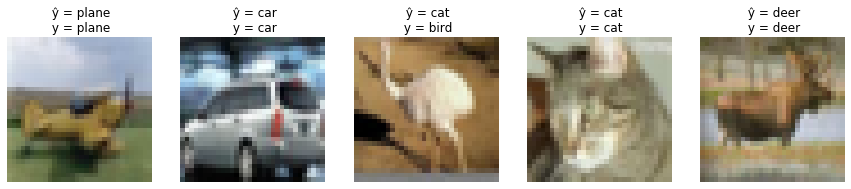
\includegraphics[width=1.\linewidth]{figures/cifar2.png}
  \caption{ {Five random samples from the CIFAR-10 dataset and their corresponding predictions and true labels using the VGG architecture. Notice how the convolutional network mistakes an ostrich (bird class) for a cat.}}
  \label{fig:cifar}
\end{figure}

Figure \ref{fig:cifar} presents five random images from the test set
and Table \ref{tab:cnn} displays results. Notice how the linear model performs poorly with just a test accuracy of 38\%, whereas increasing the flexibility of the models critically improves 
accuracy. Indeed, the MLP performs slightly better.
However, by imposing strong priors about the dataset, such as translation equivariance thanks to the convolutional layers and pooling, state-of-the-art results are achieved with VGG-19.

\begin{table}[ht]
\caption{Results over the CIFAR-10 test set.}
\centering
\begin{tabular}{ll}
Model & Test acc. \\
\hline
Linear &  $38.10\%$ \\
MLP &  $50.03\%$\\
VGG-19 &  $93.29\%$ 
\end{tabular}
\label{tab:cnn}
\end{table}

%%%%%%%%%%%%%%%
\paragraph{Transformer and recurrent models for sentiment analysis.}
This is an example with text to undertake sentiment analysis, classifying movie reviews with architectures tailored to NLP tasks. As benchmark, we use the IMBD movie review dataset 
from \parencite{maas-EtAl:2011:ACL-HLT2011}, in which a review in raw text must be classified into one of two classes: positive or negative
sentiment. 

The recurrent model consists of a LSTM network with two layers, each with hidden dimension of 256 plus a dropout of 0.5 serving as a regularizer. We also consider a simple Transformer-based model, with two encoder layers, of hidden dimension 10 plus similar dropout. For both models, the input sequence is represented as a list of one-hot encoded vectors, representing the presence of a word from a vocabulary of the 5000 most common tokens. This representation is embedded into a space of 100 dimensions
(16 in the Transformer case) by means of an affine transformation, before applying architecture-specific layers. Both models are trained using the Adam optimizer with a constant learning rate of 0.001.
%The input sequence is represented as a list of one-hot encoded vectors, representing the presence of a word from a vocabulary of the most common 5000 tokens. This discrete representation is embedded into a space of 100 dimensions (16 dimensions in the Transformer case) by means of an affine transformation, before applying the architecture-specific layers. 
%Both models are trained using the Adam optimizer with a constant learning rate of 0.001.
We also consider a bigger, transformer-based model consisting of the recent RoBERTa architecture \parencite{liu2019roberta}, 
initially pretrained on a big corpus of unsupervised raw  English text, and then fine tuned for two epochs on the IMDB training set. %As we 
 %discuss in Section \ref{sec:transfer}, pretraining with data from different tasks or domains can crucially improve the performance of Transformers, since this helps in building better representations of written language.

Table \ref{tab:examples} shows two random examples from the IMDB dataset.
Results over the full test set are displayed in Table \ref{tab:nlp}. Notice how the Transformer-based models are superior to the recurrent baseline, and the extra benefits thanks to the usage of transfer learning.

{\footnotesize
\begin{table}[ht]
\caption{Two random review samples and their corresponding predictions and true labels from the RoBERTa model.}
\centering
\begin{tabularx}{\textwidth}{Xll}
Text input & Prediction & True label \\
\hline
 {\scriptsize \texttt{HOW MANY MOVIES ARE THERE GOING TO BE IN WHICH
AGAINST ALL ODDS, A RAGTAG TEAM BEATS THE BIG GUYS
WITH ALL THE MONEY?!!!!!!!! There's nothing new in
"The Big Green". If anything, you want them to
lose. Steve Guttenberg used to have such a good
resume ("The Boys from Brazil", "Police Academy",
"Cocoon"). Why, OH WHY, did he have to do these
sorts of movies during the 1990s and beyond?! So,
just avoid this movie. There are plenty of good
movies out there, so there's no reason to waste
your time and money on this junk. Obviously, the
"green" on their minds was money, because there's
no creativity here. At least in recent years,
Disney has produced some clever movies with Pixar.} } &   Negative & Negative   \\
\hline
 {\scriptsize \texttt{When I first heard that the subject matter for
Checking Out was a self orchestrated suicide
party, my first thought was how morbid, tasteless
and then a comedy on top of that. I was skeptical.
But I was dead wrong. I totally loved it. The
cast, the funny one liners and especially the
surprise ending. Suicide is a delicate issue, but
it was handled very well. Comical yes, but tender
where it needed to be. Checking Out also deals
with other common issues that I believe a lot of
families can relate with and it does with tact and
humor. I highly recommend Checking Out. A MUST
SEE. I look forward to its release to the public.} } &   Positive & Positive   \\

\end{tabularx}
\label{tab:examples}
\end{table}
}

\begin{table}[h]
\caption{Results over the IMDB test set.}
\centering
\begin{tabular}{ll}
Model & Test acc. \\
\hline
LSTM &  $81.99\%$ \\
Simple Transformer &  $87.49\%$ \\
RoBERTa &  $94.67\%$\\
\end{tabular}
\label{tab:nlp}
\end{table}











%%%%%%%%%%%%%%%%%%

\iffalse


\subsection{Other topics}
We conclude with a discussion of three transversal topics in NN
research and applications which are gaining much traction at the moment: how may we protect the predictions of deep
learning models from malicious attacks perturbing data; how can we interpret or explain the predictions of a deep model; and, finally, how may we reuse what a deep model
learns in a domain into another related context. 

%%%%%%%%%%%%%%%%%%%%%%%%%%%%%%


\subsubsection{Explainability}

Section \ref{bayeshallow} described how the parameters 
in shallow NNs remained interpretable and this  guided
prior assessment. Explainability and interpretability are also important aspects for deep learning models,
where a decision depends on an enormous amount of weights and parameters. Here, the parameters are often abstract and disconnected from the real world, which makes it difficult to interpret and explain their results.


Thus, when properly trained, predictions obtained by
NNs may have a high accuracy but humans
often perceive the models as black boxes, their insights
remaining mostly
opaque for humans. Particularly understanding 
the entailed decision making in highly sensitive
areas such as healthcare, criminal justice, defense or finance, is of paramount importance,
requiring it to be more transparent, accountable, and understandable
for humans.
At this point is worth mentioning how the 
EU General Data Protection Regulation (GDPR) could require AI providers to deliver explanations of results of automated decision-making based on their personal data, even leading to the prohibition of the use of opaque models that are used for certain applications.

There are various approaches to the problem as 
thoroughly reviewed in ****** (2020).
One possibility is to use interpretable models,
 easily comprehensible for humans,
as cogently argued by \parencite{rudin2019stop} who claims 
that in many contexts we may perform with such models 
almost as well as with deep models.
 While using interpretable models might be appropriate for some
  contexts, they come at the cost of flexibility, accuracy, and usability.
  Alternatively, sometimes an interpretable surrogate model of the black box model is generated to gain interpretability, either globally or locally around
some test input, as with LIME \parencite{ribeiro2016model} or SHAP \parencite{lundberg2017unified}.
Finally, there are attempts to create methods for explaining 
black box models with two main broad strategies: globally
extracting an explanation from a model that is representative for some specific
data set; and locally extracting an explanation for a single test input 
 and the corresponding prediction.
  \parencite{samek2017explainable} describe different methods for visualizing and explaining deep learning models like the Layer-wise relevance propagation (LRP). 
 
 
 %%%%%%%%%%%%%%%%%%%%%%%%%%%%%%%%%%%%%%%%%
\subsubsection{Transfer learning}\label{sec:transfer}

The training of huge neural models requires large amounts of labelled data, such as images, typically in the order of thousands to millions. In cases where human labelling of training data is not feasible 
for scaling to those magnitudes, it is possible to leverage similar datasets, even not for the same task. This is called transfer learning \parencite{tan2018survey,pan2009survey}, and fundamentally consists of taking a model previously trained over a massive dataset and then fine-tune the model in the final task, with a much smaller dataset. The adoption of pretrained models allows the practitioner to save in computational costs, because it significantly shortens the training time for the final dataset, and often leads to improved performance, thanks to the already learnt knowledge of the pretrained model. In addition, the quantity of labelled data can be drastically reduced by strategically choosing the data points to be annotated. Techniques developed to automatize this idea fall under the term of active learning, and the Bayesian approach offers a principled and sound framework for it, see e.g. \parencite{houlsby2011bayesian}.

Transfer learning has enjoyed extraordinary success in fields
such as computer vision and natural language processing. With image data \parencite{girshick2014rich,NIPS2014_375c7134}, it is common to pretrain a CNN on a huge dataset (typically Imagenet, \textcite{deng2009imagenet}, with over 1M images from 1000 categories) and then use the CNN either as an initialization (this can be regarded as specifying a Bayesian prior from the previous task) or as a feature extractor for the custom task. Typically, one removes the last layer of the pretrained CNN (that which projects the hidden representation to the 1000 logits for Imagenet), and places another linear layer with softmax activations for the task of interest, or takes the hidden representation to use with another classifier, such as a support vector machine or a random forest \parencite{sharif2014cnn}. The Deep Image Prior is also an interesting example as it shows that a randomly-initialized neural network can be used as a handcrafted prior with excellent results in standard inverse problems such as denoising, super-resolution, and inpainting \parencite{ulyanov2020deep}.

Transfer learning with textual data has gained traction more recently, with the advent of gargantuan-sized language models. Models such as BERT \parencite{devlin2018bert}, or the family of GPT models \parencite{radford2018improving,radford2019language,cc:BrownMannRyderSubbiahEtAl:2020:language-models}
have achieved the state-of-the-art in many NLP tasks. 
In this case, pretraining fundamentally consists of training the Transformer with a huge amount of unsupervised data, typically scrapped from internet from sources such as Wikipedia or Common Crawl \parencite{cc:BrownMannRyderSubbiahEtAl:2020:language-models}. The pretraining task is called language modeling \parencite{2008SchpJ...3.3881B}: the model has to predict the next word in a sentence (causal language modeling), or fill in the gaps from a sentence with holes (masked language modeling). Then, one can replace the final layer of the Transformer encoder for a suitable task in order to perform finetuning to the desired task.

Tangential topics to transfer learning that are of increasing interest are meta-learning approaches such as model agnostic meta learning (MAML) \parencite{pmlr-v70-finn17a} and its Bayesian extension \parencite{NEURIPS2018_e1021d43}. Few-shot learning \parencite{wang2020generalizing}, in which a model is able to learn by providing it with only few examples per class (typically, less than 50),  has also many similitude to transfer and meta-learning. Of special interest is the extreme case of zero-shot learning, with successful applications in NLP \parencite{yinroth2019zeroshot}, and computer vision, with the example of the CLIP architecture \parencite{radford2021learning}. 
\fi


%%%%%%%%%%%%%%%%%%%%%%%%%%%%%%%%%%%%%


\subsection{Large scale Bayesian inference}

\subsubsection{Bayesian approaches}

MCMC algorithms presented in Section \ref{bayeshallow}
have become standard in Bayesian inference \cite{french}.
% Moreover, more recent variants such as HMC
% and its Riemann
%manifold variant, gain 
%some efficiency of exploration,
However, they entail a significant computational burden in large datasets. Indeed, 
computing the corresponding acceptance probabilities 
 requires iterating over the whole dataset, which often does not even
 fit into memory. Thus, they 
  do not scale well in big data settings. 
 As a consequence, two major approximations have been proposed.

%%%%%%%%%%%%%%%%%%%%
\paragraph{Stochastic Gradient Markov chain Monte Carlo}\label{bayesdeep} 

SG-MCMC methods are based on the discretization of 
stochastic differential equations that have the desired target 
distribution as its limit. \cite{ma2015complete} provide a
complete framework that encompass many earlier proposals and
facilitate such discretization, as well as a practical tool for
devising new samplers and testing the correctness of proposed samplers.

As in Section 2.2, we aim at drawing samples from the
posterior $p(\theta |D) \propto \exp(-U(\theta ))$,
with potential function
$U(\theta ) = -\sum _{x\in D} \log p(x|\theta ) + \log p(\theta )$. Define also auxiliary variables $r$,
with $z=( \theta, r )$, and sample from $p(z|D) \propto  \exp(-H(z))$, with hamiltonian
$H(z) = H(\theta , r) = U(\theta ) + g(\theta , r)$, such that
$\exp(-g(\theta , r))dr = constant$. 
Marginalizing the auxiliary variables gives us the desired distribution on $\theta $.

In general, all continuous Markov processes that one might consider for sampling can be written
as a stochastic differential equation (SDE) of the form:
\begin{equation}
dz = f(z)dt +
\sqrt{ 2D(z)}dW(t),
\end{equation}
where $f(z)$ denotes the deterministic drift, frequently
related to $\nabla H(z)$,
$W(t)$  is a $d$-dimensional Wiener process, and 
$D(z)$ is a positive semidefinite diffusion matrix. Note, though,
that some care must be taken to choosing $f(z)$ and $D(z)$ 
to yield the desired stationary distribution.
\cite{ma2015complete} propose a recipe for constructing SDEs with the correct stationary distribution through 
$f(z) = - [D(z) + Q(z)] \nabla H(z) + \Gamma (z)$, 
and $\Gamma _i (z) = \sum _{j=1}^d 
\frac{\partial  }{\partial z_j}(D_{ij} (z) + Q_{ij} (z) )
$
where $ Q(z)$ is a skew-symmetric curl matrix (representing the deterministic traversing effects seen
in HMC procedures) and the diffusion matrix $D(z)$
determines the strength of the Wiener process-driven diffusion.
When 
$D(z)$ is positive semidefinite and $Q(z)$ is skew-symmetric, 
 the convergence of the above dynamics to the desired 
distribution follows; moreover both matrices can be adjusted to attain faster convergence to
the posterior distribution. \cite{ma2015complete} show that by properly choosing the matrices  one can recover numerous samplers such
as SGLD \cite{welling2011bayesian} or a corrected SG-HMC \cite{chen2014stochastic}.

In practice, simulation actually relies on a discretization of the SDE, leading to a (full-data) update rule
\begin{equation}
z_{t+1} \leftarrow z_t - \epsilon_t \left[ ( D(z_t) + Q(z_t) )
\nabla H(z_t) + \Gamma (z_t)\right]
+ N (0, 2\epsilon _t D(z_t)).
\end{equation} 
Calculating $\nabla H(z)$ entails evaluating the gradient of $U(\theta )$
which, with deep NN models, 
 becomes very intensive computationally as it relies on a sum
over all data points. Instead, 
we use a sampled data subset $S' \subset S$, with the corresponding potential for these data being 
$U_1 (\theta ) = -\frac{|S'|}{|S|} \sum _{x \in S'}
\log p(x|\theta ) + \log p(\theta )$, leading 
to the approximation 
\begin{equation}
z_{t+1} \leftarrow z_t - \epsilon_t \left[ ( D(z_t) + Q(z_t) )
\nabla H (z_t) + \Gamma (z_t) \right]
+ N (0, \epsilon _t (2 D(z_t)- \epsilon_t \hat {B_t}))
\end{equation} 
where $\hat {B_t}$ is an estimate of the variance of the error.
This provides the  stochastic gradient—or minibatch— variant of the sampler. 


%%%%%%%%%%%%%%%%%%%%%
\paragraph{Variational Bayes} 

Variational inference (VI) \cite{blei2017variational} tackles the 
 approximation of  $p(\theta | D)$ with a tractable parameterized
 distribution $q_{\phi}(\theta |D)$. The goal is to find parameters $\phi$ so that the distribution 
$q_{\phi}(\theta |D )$  (referred to as variational guide
or variational approximation)  is as close as possible to the actual posterior, with closeness typically measured through 
the Kullback-Leibler 
divergence $KL(q_{\phi } || p)$, reformulated into the ELBO
\begin{equation}\label{eq:elbo}
\mbox{ELBO}(q) = \mathbb{E}_{q_{\phi}(\theta |D)} \left[ \log p(D,\theta ) - \log q_{\phi}(\theta |D)\right],
\end{equation}
the objective to be optimized,
usually through SGD techniques. 

A standard choice
for $q_{\phi}(\theta |D )$ is a factorized Gaussian 
distribution $\mathcal{N}(\mu_{\phi}(D), \sigma_{\phi}(D))$,
with  mean and covariance matrix defined through a
 deep NN conditioned on the observed data $D$.
 Note though that 
other distributions can be adopted as long as they 
 are easily sampled and their log-density and entropy evaluated. 
A problem is that these approximations often 
underestimate the uncertainty. Some developments
partly mitigate this  issue
by  enriching the variational family include normalizing flows \cite{rezende2015variational} or the use of implicit distributions \cite{huszar2017variational}.

We can actually use a more flexible approximation \cite{VIS},
 designated {\em refined variational approximation}, 
  by embedding a sampler (Section 3.3.1) through
\begin{equation*}\label{eq:q}
q_{\phi,\eta}(\theta |D) = \int Q_{\eta, T}(\theta  | \theta _0)q_{0,\phi}(\theta _0|D)d\theta _0,
\end{equation*}
where $q_{0,\phi} (\theta | D)$ is the initial and tractable density
$q_{\phi} (\theta | D)$.  
The conditional distribution $Q_{\eta, T}(\theta |\theta _0)$
designates a stochastic process parameterized by $\eta$,  
used to evolve the original density $q_{0,\phi}(\theta |D )$
for $T$ periods, so as to achieve greater flexibility. 
 Observe that when $T=0$, no refinement steps are performed and the refined variational approximation coincides with the original one; on the other hand, as 
 $T$ increases, the approximation will be closer to the exact posterior, assuming that $Q_{\eta, T}$ is a valid sampler
 as in Section \ref{bayesdeep}. Specific 
forms for $Q_{\eta, T}(\theta |\theta _0)$
are described in \cite{VIS}.
We next maximize a refined ELBO objective, replacing in (\ref{eq:elbo}) the 
original $q_{\phi }$ 
by $q_{\phi, \eta}$
\begin{equation}\label{eq:ELBO}
\mbox{ELBO}(q_{\phi,\eta}) = \mathbb{E}_{q_{\phi, \eta}(\theta D)}
\left[ \log p(D, \theta ) - \log q_{\phi, \eta}(\theta |D)\right]
\end{equation}
to optimize the divergence $KL(q_{\phi,\eta}(\theta |D) ||  p(\theta |D ))$. 
%{\bf{The first term of Eq. (\ref{eq:ELBO})}}
%requires only being able to sample from $q_{\phi,\eta}(z|x)$; however the second
%one, the entropy
%$-\mathbb{E}_{q_{\phi,\eta}(z|x)} \left[ \log q_{\phi,\eta}(z | x) \right]$, requires also evaluating the evolving, implicit density.
%Section 3.2 describes 
Efficient methods to approximate 
 such 
evaluation are available in \cite{VIS}. 

As a consequence, performing variational inference with the refined variational approximation can be regarded as using the original variational guide while optimizing an alternative, tighter ELBO.  
This facilitates a framework for learning the sampler parameters $\phi, \eta$ using gradient-based optimization based 
on two phases: first,
 refinement, sampler parameters are learnt in an optimization loop that maximizes the ELBO with the new posterior;
after several iterations, the inference  phase 
starts and we just let the tuned sampler run for
sufficient iterations as used in SG-MCMC samplers. Algorithmically,
this is expressed as in Algorithm \ref{alg:vis}.
\iffalse
{\tt 
\begin{description}
    \item[Refinement phase] Repeat until convergence:
    \begin{enumerate}
    \item Sample initial set of particles, $\theta _0 \sim q_{0,\phi}(\theta | D)$.
    \item Refine particles through sampler, $\theta _T \sim Q_{\eta, T}(\theta |\theta 0)$.
    \item Compute the ELBO objective (\ref{eq:ELBO}). 
    \item Update parameters $\phi, \eta$ through automatic 
    differentiation on objective.
\end{enumerate}
    \item[Inference phase] Based on learnt sampler parameters $\phi^*, \eta^*$:
    \begin{enumerate}
    \item Sample an initial set of particles, $\theta _0 \sim q_{0,\phi^*}(\theta |D)$.
    \item Use the MCMC sampler $\theta _T \sim Q_{\eta^*, T}(\theta |\theta _0)$ as $T \rightarrow \infty$.
    \end{enumerate}
\end{description}
}

{\tt
\begin{algorithm}[H]
Refinement phase: \\
\While{not convergence}{
 Sample initial set of particles, $\theta _0 \sim q_{0,\phi}(\theta | D)$. \\
 Refine particles through sampler, $\theta _T \sim Q_{\eta, T}(\theta |\theta 0)$. \\
 Compute the ELBO objective (\ref{eq:ELBO}).  \\
 Update parameters $\phi, \eta$ through automatic 
    differentiation on objective. \\
 }

Inference phase. Based on learnt sampler parameters $\phi^*, \eta^*$:\\
\quad Sample an initial set of particles, $\theta _0 \sim q_{0,\phi^*}(\theta |D)$. \\
\quad  Use the MCMC sampler $\theta _T \sim Q_{\eta^*, T}(\theta |\theta _0)$ as $T \rightarrow \infty$.
 \caption{VIS sampler}\label{alg:vis}
\end{algorithm}
}
\fi

%%%%%%%%%%%%%%%%%%%%%%%
\paragraph{Ensembles} \cite{bdl} showed that deep ensembles \cite{ensemble} provide an efficient technique for approximate Bayesian marginalization, although it is not a truly Bayesian method.

A regularization technique called dropout can be interpreted as performing ensembling over several models \cite{dropout}. Motivated by how dropout could be effectively used to quantify uncertainty in deep networks \cite{pmlr-v48-gal16}, several explorations have been pursued to extend ensembles for similar purposes. Deep ensembles were found to be superior to MC dropout in out-of-distribution-settings \cite{Ovadia2019CanYT}.
Some recent techniques that should be pointed out include
Stochastic Weight Averaging (SWA) \cite{izmailov2018averaging}, which leads to much more robust optima and better generalization, and a Bayesian treatment of the previous approach based on a Gaussian distribution,
called SWAG \cite{NEURIPS2019_118921ef}.

Stein Variational Gradient Descent (SVGD) \cite{svgd} takes a set of particles and evolves it following the gradient of the loss plus an auxiliary term that acts as a repulsion force between particles. That
way, the particles do not collapse into the same mode, and can explore wider areas of the posterior. There is a close relationship between SVGD and SG-MCMC methods with \cite{gallego2018stochastic} 
studying the interaction between both methods.

Deep learning ensemble applications abound, for example in probabilistic wind power forecasting \cite{wang2017deep}, speech recognition \cite{deng2014ensemble}, time series forecasting \cite{qiu2014ensemble}, and medicine or bioinformatics \cite{qummar2019deep,xiao2018deep,cao2020ensemble}. However, the vast majority of these applied works only use simple ensembles, by averaging the outputs. Further benefits could be achieved by realizing a full Bayesian treatment of the problem.


\paragraph{Final remarks}
Lastly, note that all of these approaches could be combined with recent heuristics to improve the convergence of SGD methods, such as the adoption of cyclical learning rates to explore more efficiently the posterior  \cite{7926641}.


%%%%%%%%%%%%%%%%%%%%%
%%%%%%%%%%%%%%%%%%%%%%%%%%%%%%%%%%%



\subsection{Security of machine learning}


As described, over the last decade
an increasing number of processes are being automated through 
deep NN algorithms, being 
essential that these are robust and reliable
if we are to
trust operations based on their output. State-of-the-art
algorithms, as those described above, perform extraordinarily well on standard data,  but have been
shown to be vulnerable to adversarial examples, data instances targeted at
fooling them \cite{goodfellow2014explaining}.
The presence of adaptive adversaries has
been pointed out in areas such as spam detection \cite{zeager2017adversarial}
and computer vision \cite{goodfellow2014explaining}, among many others. 
In those contexts, algorithms should acknowledge the presence of possible adversaries
to protect from their data manipulations.
As a fundamental underlying hypothesis, NN
based systems rely on using 
independent and identically distributed (iid) data for both training and operations. However, security aspects in deep
learning, part of the emergent field of
adversarial machine learning (AML),
question such hypothesis, given the
presence of adaptive adversaries ready to  intervene in the problem 
to modify the data and obtain a benefit. 

As a motivating example, vision algorithms (Section
\ref{kkvision}) are at the core of many AI 
applications such as ADSs \cite{rumanos}. 
The simplest and most notorious attack examples to
such algorithms  
consist of modifications of images in such a way that the alteration becomes imperceptible to the human eye, yet drives a model trained on millions of images to misclassify the modified ones,
with potentially relevant security consequences.
With a relatively simple CNN model (Section 3.1.1), we are able to accurately predict 99\% of the handwritten digits in the MNIST data set.
However, if we attack those data with the fast gradient sign method \cite{szegedy2013intriguin},
accuracy gets reduced to 62\%. Fig.~\ref{fig:digits} provides an example of an original MNIST image and a perturbed one: to our eyes both images look like a 2, but the classifier rightly identifies a 2 in the first case, whereas it suggests a 7 after the perturbation. 
%
%\vspace{-0.2in}
%
%\hfill $\triangle$
%
\begin{figure}[hbt]
\centering
  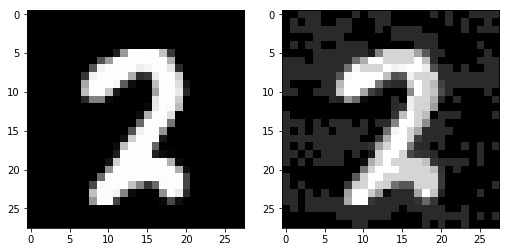
\includegraphics[width=.6\linewidth]{figures/27}
  \caption{Left: original image, correctly classified as a 2. Right: slightly perturbed image, wrongly classified as a 7.}
  \label{fig:digits}
\end{figure}

Stemming from the pioneering work in adversarial classification 
\cite{adversarialClassification2004}, the prevailing paradigm in AML models
the confrontation between learning-based systems and adversaries through game theory. 
This entails common knowledge assumptions 
\cite{hargreaves2004game} which are 
questionable in security 
applications as adversaries try to conceal information. 
As \cite{fan2019selective} points out, there is a need for a  framework that guarantees robustness of ML against adversarial manipulations in a principled manner. 

The usual approach for robustifying models against these examples is {\em adversarial training} (AT) \cite{madry2018towards} and its 
variants, based on solving a 
bi-level optimisation problem whose objective function is the empirical risk of a model under worst case data perturbations. % AT approximates the inner optimisation through a projected gradient descent  
%algorithm, ensuring that the perturbed input falls within a tolerable boundary, usually specified through some restriction on a norm distance. 
However, recent pointers urge modellers to depart from using 
norm based approaches \cite{carlini2019evaluating} and develop more realistic attack models.

AML is a  difficult area which rapidly evolves and leads to an 
arms race in which the community alternates cycles of proposing attacks and  of implementing defences that deal with them. However, as mentioned, it is 
based on game theoretic ideas and strong common
knowledge conditions. 
\cite{AMLARA} propose a
Bayesian decision theoretic based methodology 
to solve AML problems, 
adopting an ARA perspective \cite{adversarialRiskAnalysis2009,banks2015adversarial} modeling the confrontation between attackers and defenders and mitigating questionable common knowledge assumptions. \cite{math8111957} applies this ARA-based framework to  adversarial classification.

%%%%%%%%%%%%%%%%%%%%%%%%%%%%%%%%




\subsection{Large scale competitive decision making}


Relacionar cada uno con \ref{sec:dlms}.


\section{Thesis structure}